\documentclass[12pt, a4paper, twoside]{article}
\usepackage[margin=1in, headheight=0.3in, headsep=0.2in]{geometry}
\textwidth 16.5 cm \textheight 24cm
\oddsidemargin -2mm

% Packages
\usepackage{amsmath, listings, xcolor, tcolorbox, microtype, fancyhdr, hyperref, tikz, float}
\usetikzlibrary{decorations.pathreplacing}

% Configure text justification
\raggedbottom
\renewcommand{\textfraction}{0.05}
\renewcommand{\floatpagefraction}{0.85}
\renewcommand{\topfraction}{0.9}

% Configure the header
\setlength{\headheight}{14.49998pt}
\pagestyle{fancy}
\fancyhf{} 
\fancyhead[L]{\leftmark}
\fancyhead[R]{\thepage}
\renewcommand{\footrulewidth}{0pt}
\renewcommand{\sectionmark}[1]{\markboth{\thesection.~#1}{}}
\renewcommand{\subsectionmark}[1]{}

\newcommand{\be}{\begin{equation*}}
\newcommand{\ee}{\end{equation*}}

% Configure the links to look professional
\hypersetup{
    colorlinks=true,      % false: boxed links; true: colored links
    linkcolor=navyblue,   % Color of internal links (TOC, sections)
    citecolor=navyblue,   % Color of citations
    urlcolor=navyblue,    % Color of external URLs
    pdftitle={Numerical Solutions using WKB},  % Metadata for the PDF
    pdfauthor={Mohak Das}                      % Metadata for the PDF
}

% Define custom colors for code
\definecolor{codegreen}{rgb}{0,0.6,0}
\definecolor{codegray}{rgb}{0.5,0.5,0.5}
\definecolor{codepurple}{rgb}{0.58,0,0.82}
\definecolor{backcolour}{rgb}{0.95,0.95,0.92}
\definecolor{navyblue}{RGB}{0, 51, 102} % A professional deep blue

% Configure the Fortran style
\lstdefinestyle{codestyle}{
    backgroundcolor=\color{backcolour},   
    commentstyle=\color{codegreen},
    keywordstyle=\color{magenta},
    numberstyle=\tiny\color{codegray},
    stringstyle=\color{codepurple},
    basicstyle=\ttfamily\footnotesize, % Typewriter font, small size
    breakatwhitespace=false,         
    breaklines=true,                 % Break long lines automatically
    captionpos=b,                    % Caption at bottom
    keepspaces=true,                 
    numbers=left,                    % Line numbers on the left
    numbersep=5pt,                  
    showspaces=false,                
    showstringspaces=false,
    showtabs=false,                  
    tabsize=4,
    language=Fortran                 % Set language to Fortran
    }
    
% Configure the Python style
\lstdefinestyle{mypython}{
    language=Python,
    backgroundcolor=\color{backcolour},   
    basicstyle=\ttfamily\footnotesize,
    keywordstyle=\color{blue},
    stringstyle=\color{red},
    commentstyle=\color{green!60!black},
    numberstyle=\tiny\color{codegray},
    breakatwhitespace=false,         
    breaklines=true,                 % Break long lines automatically
    captionpos=b,                    % Caption at bottom
    keepspaces=true,                 
    numbers=left,                    % Line numbers on the left
    numbersep=8pt,                  
    showspaces=false,                
    showstringspaces=false,
    showtabs=false,                  
    tabsize=4,
} 

% Define a style for raw text output
\lstdefinestyle{outputstyle}{
    backgroundcolor=\color{white},   
    basicstyle=\ttfamily\small,      % Monospaced font
    breaklines=true,                 % Wrap long lines
    frame=single,                    % Add a black frame around the output
    numbers=none,                    % No line numbers
    captionpos=b,
    keepspaces=true
}

\begin{document}

    \begin{titlepage}
        \centering

        \vspace*{\fill}
        \Huge \textsc{\textcolor{navyblue}{Jadavpur University}}\\
        \LARGE \textsc{Department of Physics}\\[1cm]

        \textcolor{navyblue}{\rule{\linewidth}{0.8mm}} \\[0.4cm] 
        \Huge \textbf{\textcolor{navyblue}{Numerical Solutions using the \\ Finite Difference Method}} \\[0.2cm]
        \textcolor{navyblue}{\rule{\linewidth}{0.8mm}} \\[1.5cm] 

        \large \textit{The Discretization Scheme}\\[0.5cm]

        \begin{tcolorbox}[colback=navyblue!5!white, colframe=navyblue, width=0.8\textwidth, boxrule=0.5mm, arc=2mm, auto outer arc]
            \centering \Large
            $$\frac{d^2\psi_i}{dx^2} \approx \frac{\psi_{i+1} - 2\psi_i + \psi_{i-1}}{\Delta x^2}$$
        \end{tcolorbox}

        \vspace{1.5cm}

        \noindent
        \begin{minipage}{0.4\textwidth}
            \begin{flushleft} \Large
                \textbf{Submitted by:}\\
                \textcolor{navyblue}{Mohak Das}\\
            \end{flushleft}
        \end{minipage}
        \begin{minipage}{0.4\textwidth}
            \begin{flushright} \Large
                \textbf{Supervisor:} \\
                Dr. Asim Kumar Ghosh\\
                \vspace{0.6cm}
            \end{flushright}
        \end{minipage}
        \vspace{1cm}

        \textbf{Class:} PG-I\\
        \textbf{Class Roll No:} 002520702028\\
        \textbf{Exam Roll No:} PPHD0261034
        \vspace{1.5cm}

        \textsc{Computational Physics Lab}

        \vspace*{\fill}


    \end{titlepage}
    \thispagestyle{empty}

    \begin{abstract}
        This report presents a comprehensive numerical investigation of the 1D Time-Independent Schrödinger Equation (TISE) utilizing the Finite Difference Method (FDM). The continuous differential equation was discretized into a symmetric tridiagonal matrix eigenvalue problem and solved efficiently using the TQLI (Tridiagonal QL Implicit) algorithm implemented in Fortran. A diverse suite of fourteen distinct quantum potentials was analyzed, ranging from foundational models—such as the infinite square well and harmonic oscillator—to complex anharmonic, asymmetric, and coupled-well systems. Furthermore, the computational methodology was extended to advanced physical applications, successfully modeling molecular dissociation via the Morse potential and singular boundary behavior via the Dirac-delta potential. Data visualization, handled systematically in Python, shifted the computed wavefunctions by their respective discrete eigen-energies. This approach provided clear visual confirmations of core quantum mechanical phenomena, including parity alternation, quantum penetration into classically forbidden regions, tunneling-induced spontaneous symmetry breaking, and the strict numerical distinction between bound and scattering states.
    \end{abstract}
    
    \thispagestyle{empty}
    \newpage

  	\tableofcontents
	\thispagestyle{empty}
	
	\clearpage
	\pagenumbering{arabic}

    \section{Introduction}

        \subsection{Main Idea}
        Analytically solving the 1D Time-Independent Schrödinger Equation (TISE) is only possible for a handful of idealized potentials, such as the infinite square well or the simple harmonic oscillator. For arbitrary or complex potentials, exact analytical solutions do not exist. To study these systems, we must rely on numerical approximations. The Finite Difference Method (FDM) provides a robust framework for this by converting the continuous differential equation into a discrete algebraic eigenvalue problem that computers can solve efficiently. It is particularly powerful because it can handle any potential shape simply by evaluating the potential function at discrete spatial points.

        \subsection{Derivation and Discretization}
        We begin with the 1D Time-Independent Schrödinger Equation:

        $$-\frac{\hbar^2}{2m} \frac{d^2\psi(x)}{dx^2} + V(x)\psi(x) = E\psi(x)$$

        To discretize this, we divide the spatial domain into $N$ equally spaced grid points with a step size of $\Delta x$. Let $x_i$ be the position of the $i$-th grid point, and $\psi_i = \psi(x_i)$ be the wavefunction value at that point.Using the central difference approximation for the second derivative, we get:
        
        $$\frac{d^2\psi_i}{dx^2} \approx \frac{\psi_{i+1} - 2\psi_i + \psi_{i-1}}{\Delta x^2}$$
        
        Substituting this back into the TISE yields the discrete equation for each grid point $i$:
        
        $$-\frac{\hbar^2}{2m \Delta x^2} (\psi_{i+1} - 2\psi_i + \psi_{i-1}) + V(x_i)\psi_i = E\psi_i$$

        \subsection{Matrix Formulation}
        Grouping the terms by $\psi_{i-1}$, $\psi_i$, and $\psi_{i+1}$, we can rewrite the equation as:
        
        $$\left( \frac{\hbar^2}{2m \Delta x^2} + V(x_i) \right) \psi_i - \frac{\hbar^2}{2m \Delta x^2} \psi_{i+1} - \frac{\hbar^2}{2m \Delta x^2} \psi_{i-1} = E\psi_i$$
        
        This forms a system of linear equations. Considering $\psi_0 = \psi_{N+1} = 0$ (Dirichlet Boundary conditions), the above set of linear equations can be written in a matrix equation form:
        \be
        \boxed{\begin{pmatrix}
        2K + V(x_1) & -K & 0 & \cdots & 0 \\
        -K & 2K + V(x_2) & -K & \cdots & 0 \\
        0 & -K & 2K + V(x_3) & \cdots & 0 \\
        \vdots & \vdots & \vdots & \ddots & \vdots \\
        0 & 0 & 0 & \cdots & 2K + V(x_N)
        \end{pmatrix}
        \begin{pmatrix}
        \psi_1 \\
        \psi_2 \\
        \psi_3 \\
        \vdots \\
        \psi_N
        \end{pmatrix}
        = E
        \begin{pmatrix}
        \psi_1 \\
        \psi_2 \\
        \psi_3 \\
        \vdots \\
        \psi_N
        \end{pmatrix}}
        \ee
        where $K = \frac{\hbar^2}{2m \Delta x^2}$
        \begin{itemize}
            \item Main Diagonal Elements ($d_i$): $d_i = \frac{\hbar^2}{m \Delta x^2} + V(x_i)$ 
            \item Off-Diagonal Elements ($e_i$): $e_i = -\frac{\hbar^2}{2m \Delta x^2}$
        \end{itemize}
        

    \section{Numerical Implementation}

        \subsection{Global Constants and Precision}
        To ensure numerical stability and physical consistency across all problems, a shared module \texttt{constants\_mod} is used. This module defines the double-precision floating-point kind (\texttt{real64}) and sets the atomic units ($\hbar = 1, m = 1$).

        \lstinputlisting[caption={Global Constants Module}, style= codestyle, label={lst:const}]{src/shared/constants_mod.f90}

        \subsection{The General FDM Solver}
        The core logic is encapsulated in the \texttt{FDM\_toolbox} module.
        To diagonalize the Hamiltonian matrix, the TQLI (Tridiagonal QL Implicit) algorithm was implemented. Standard eigenvalue solvers (like the Jacobi method) require $O(N^3)$ operations, which becomes computationally prohibitive for large grids. TQLI exploits the tridiagonal nature of our specific matrix, finding eigenvalues in highly efficient $O(N^2)$ time using Givens rotations and Wilkinson shifts to accelerate convergence. To organize the results physically, a custom \texttt{sort\_eigen} subroutine was used to arrange the eigenvalues in ascending order ($E_0 < E_1 < E_2 \dots$), simultaneously rearranging the corresponding eigenvector columns to maintain the correct energy-state pairings.

        \lstinputlisting[caption={FDM Toolbox Implementation}, style= codestyle, label={lst:solver}]{src/shared/FDM_toolbox.f90}

        \subsection{Data Visualization (Python Setup)}
        To clearly visualize the quantum states and their classical turning points, the wavefunctions were scaled by a visual factor and shifted by their corresponding energy eigenvalues ($E_n$). The following generalized Python script serves as the core visualization template for all problems. For each specific potential, placeholders such as the input file, energy list, and scale factor were dynamically adjusted.

        \begin{lstlisting}[style=mypython]
        import numpy as np
        import matplotlib.pyplot as plt

        # --- Configuration Placeholders ---
        DATA = np.loadtxt("data/<FILENAME>.dat")
        ENERGIES = np.loadtxt("data/<FILENAME>_energies.dat") # Eigenvalues from Fortran solver
        SCALE_FACTOR = <VALUE> # Visual scaling to prevent wavefunction overlap

        # --- Data Loading ---
        # Columns: x, V(x), psi_0, psi_1, psi_2, ...
        x = DATA[:, 0]
        V_x = DATA[:, 1]

        # Extract wavefunctions dynamically based on the number of energies provided
        wavefunctions = [DATA[:, i] for i in range(2, len(ENERGIES) + 2)]

        # --- Visualization ---
        plt.figure(figsize=(8, 8))

        # Plot the background potential
        plt.plot(x, V_x, color='black', linewidth=2, label='V(x)')

        # Plot shifted and scaled wavefunctions
        for n, (psi, E) in enumerate(zip(wavefunctions, ENERGIES)):
            plt.plot(x, (psi * SCALE_FACTOR) + E, label=f'n={n} (E={E:.4f})')
            plt.axhline(E, color='gray', linestyle='--', alpha=0.5) # Energy level guide

        # Formatting
        plt.title("<PROBLEM_TITLE>", size=15)
        plt.xlabel(r'Position $(x)$', size=15)
        plt.ylabel(r'Wavefunction $\psi(x)$', size=15)
        plt.xlim(<X_MIN>, <X_MAX>)
        plt.ylim(<Y_MIN>, <Y_MAX>)

        # Push legend outside the right edge of the plot
        plt.legend(loc='upper center', bbox_to_anchor=(0.5, -0.15), ncol=3)
        plt.subplots_adjust(bottom=0.2)
        plt.tight_layout()
        plt.show()
        \end{lstlisting}

    
    \section{Solution to the Assignment Problems}
        \subsection{Problem 1: Slanted Base Infinite Potential Well}
        \begin{itemize}
            \item {\bf Description: } An infinite well where the floor is not flat, but slopes upwards linearly.
            \item {\bf Potential: } $V(x) = \frac{V_0}{L}x$ for $0 \le x \le L$, and $\infty$ elsewhere. $V_0 = 200$, $L = 1$.
            \item {\bf Code: } \lstinputlisting[style= codestyle]{src/problems/prob01_infinite_potential_well_slanted_base.f90}
            \item {\bf Output: } \lstinputlisting[style= outputstyle]{output/prob01.txt}
            \item {\bf Plot: }The wavefunctions were visualized using the standard scaling script (defined in Section 2.3) with a visual \texttt{scale\_factor} of 300.0 to prevent overlap between the energy levels.\begin{figure}[H]
            \centering
            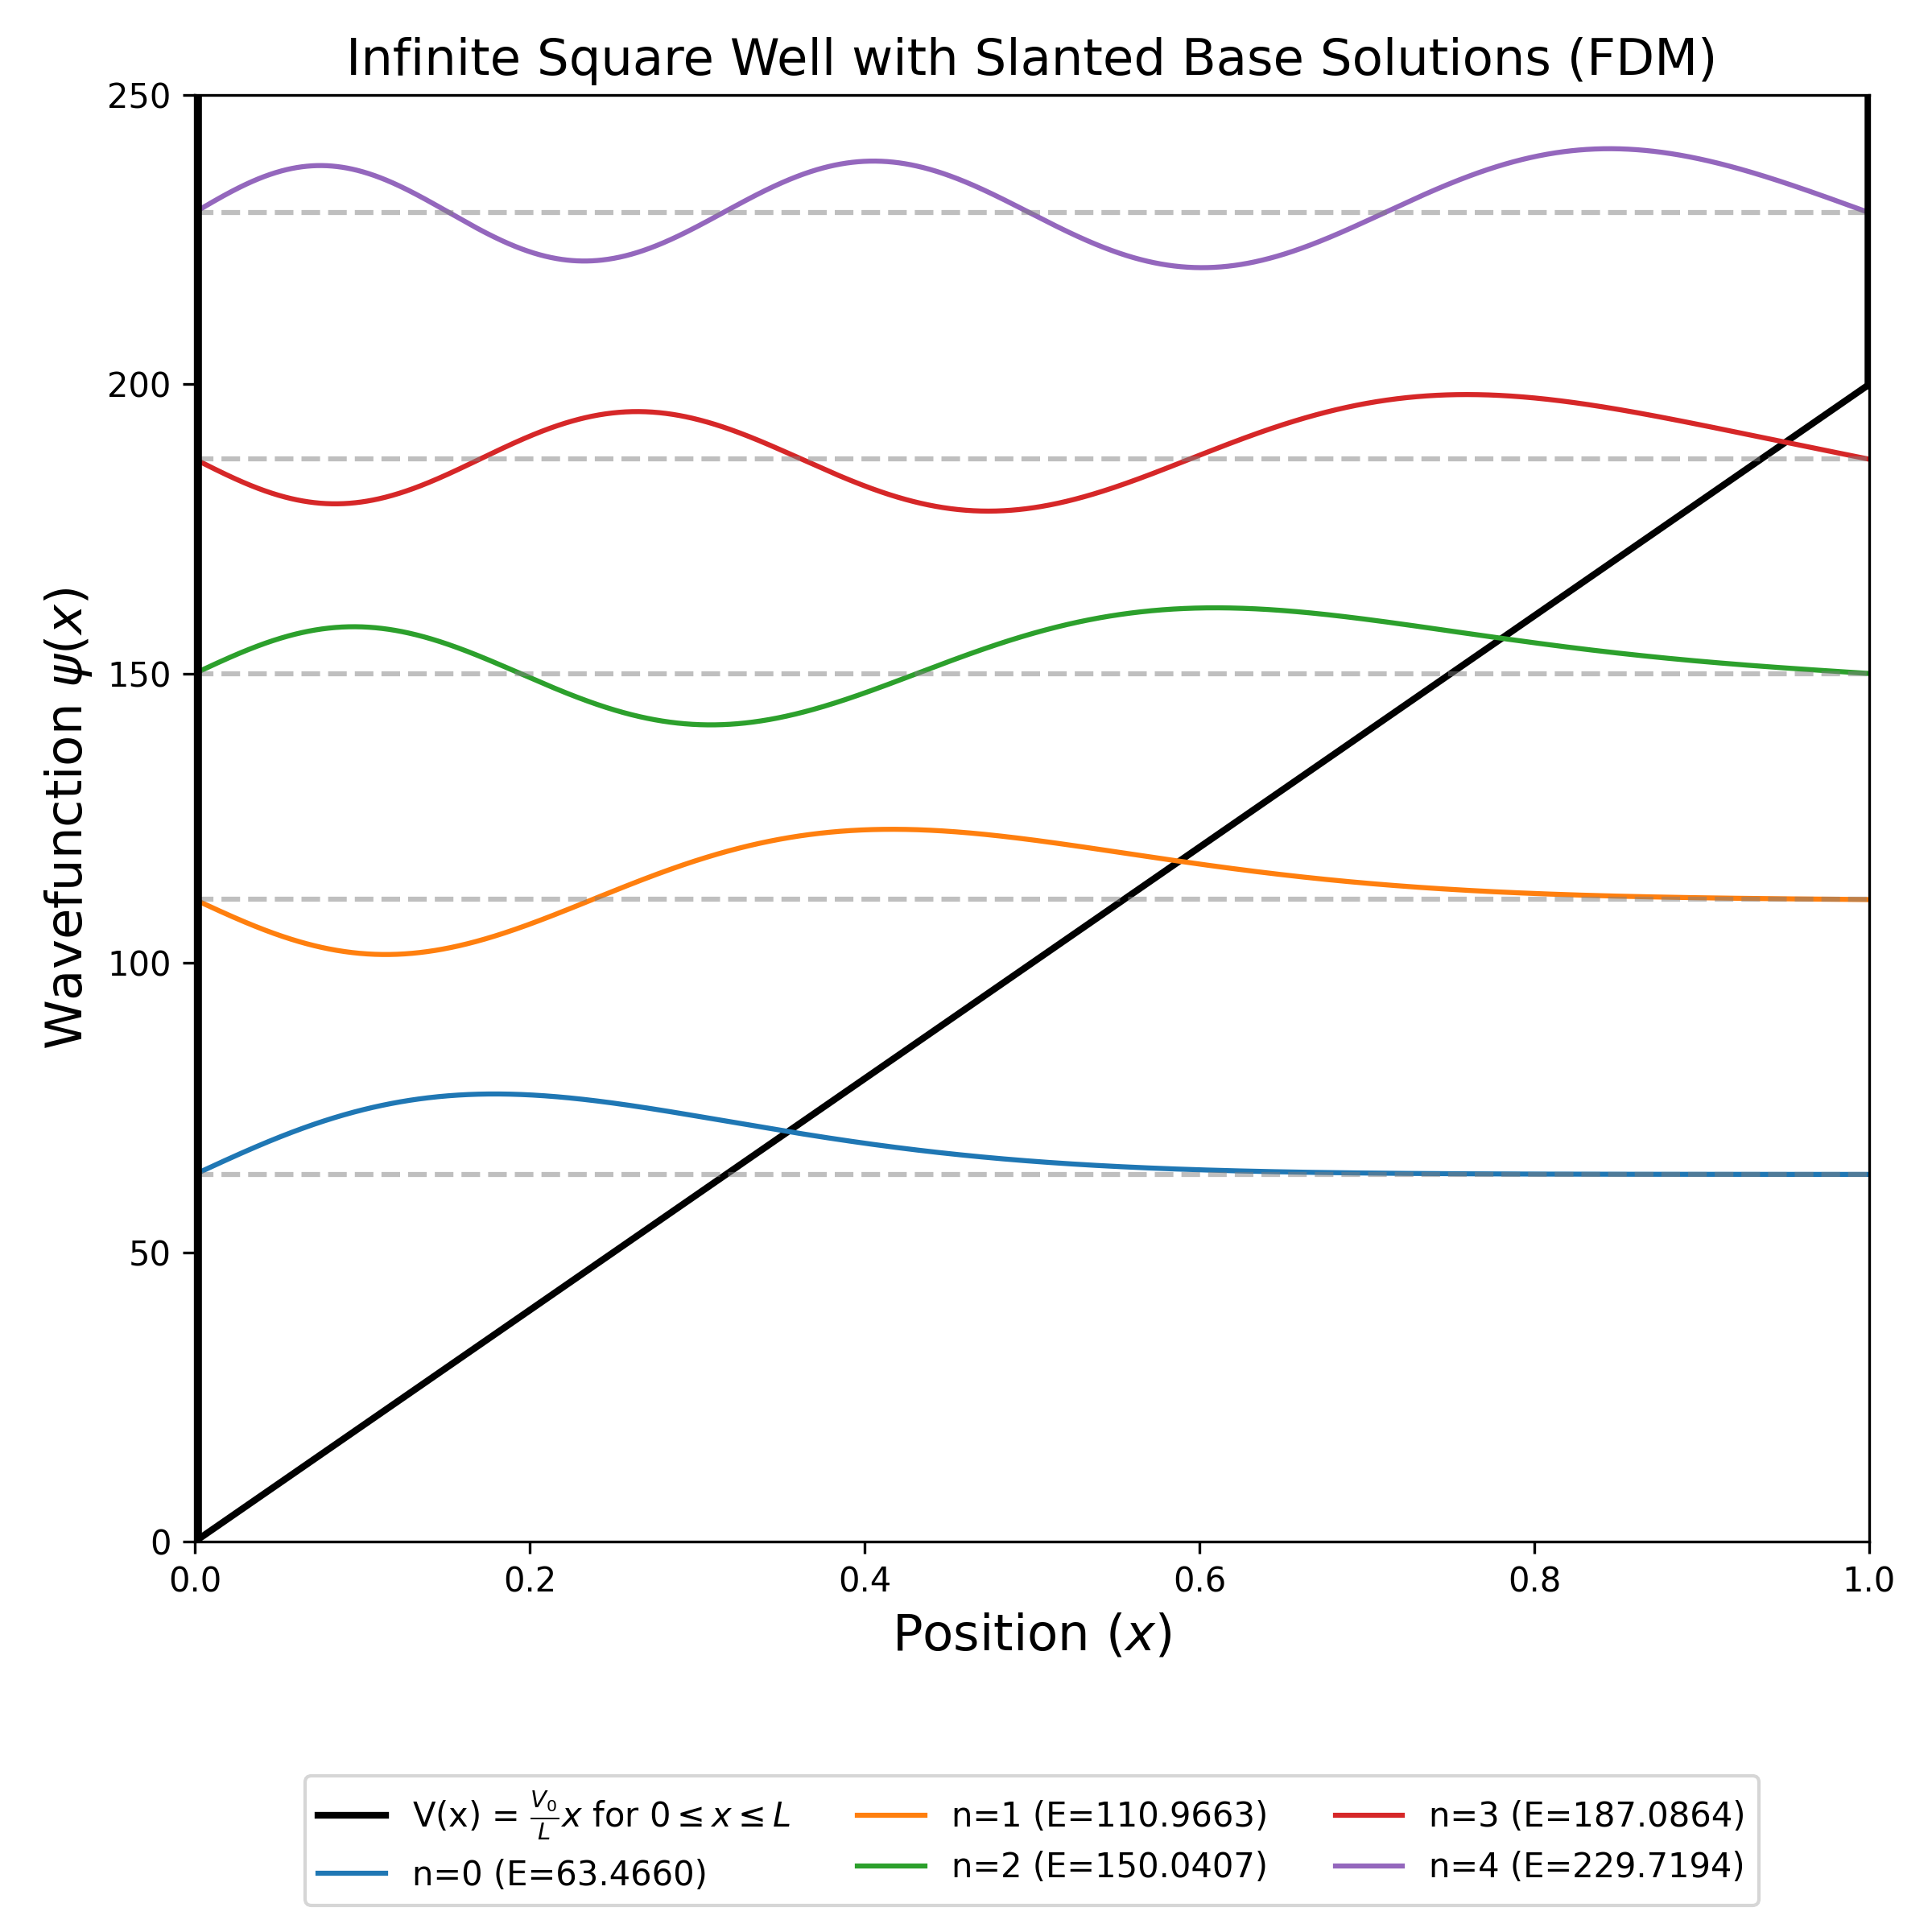
\includegraphics[width=0.8\textwidth]{plots/prob01_infinite_square_well.png}
            \label{fig:prob01_wavefunction}
            \end{figure}
            \item {\bf Plot Analysis: } Unlike the standard square well, the wavefunctions are pushed towards the lower-potential side (left side). The symmetry is broken, and the expectation value of position $\langle x \rangle$ shifts toward $x=0$.
        \end{itemize}

        \subsection{Problem 2: One-dimensional Half-Harmonic Potential}
        \begin{itemize}
            \item {\bf Description: } A harmonic oscillator cut in half by an infinite wall at the origin.
            \item {\bf Potential: }  $V(x) = \frac{1}{2}m\omega^2 x^2$ for $x \ge 0$, and $\infty$ otherwise.
            \item {\bf Code: } \lstinputlisting[style= codestyle]{src/problems/prob02_half_harmonic.f90}
            \item {\bf Output: } \lstinputlisting[style= outputstyle]{output/prob02.txt}
            \item {\bf Plot: }The wavefunctions were visualized using the standard scaling script (defined in Section 2.3) with a visual \texttt{scale\_factor} of 10.0 to prevent overlap between the energy levels.\begin{figure}[H]
            \centering
            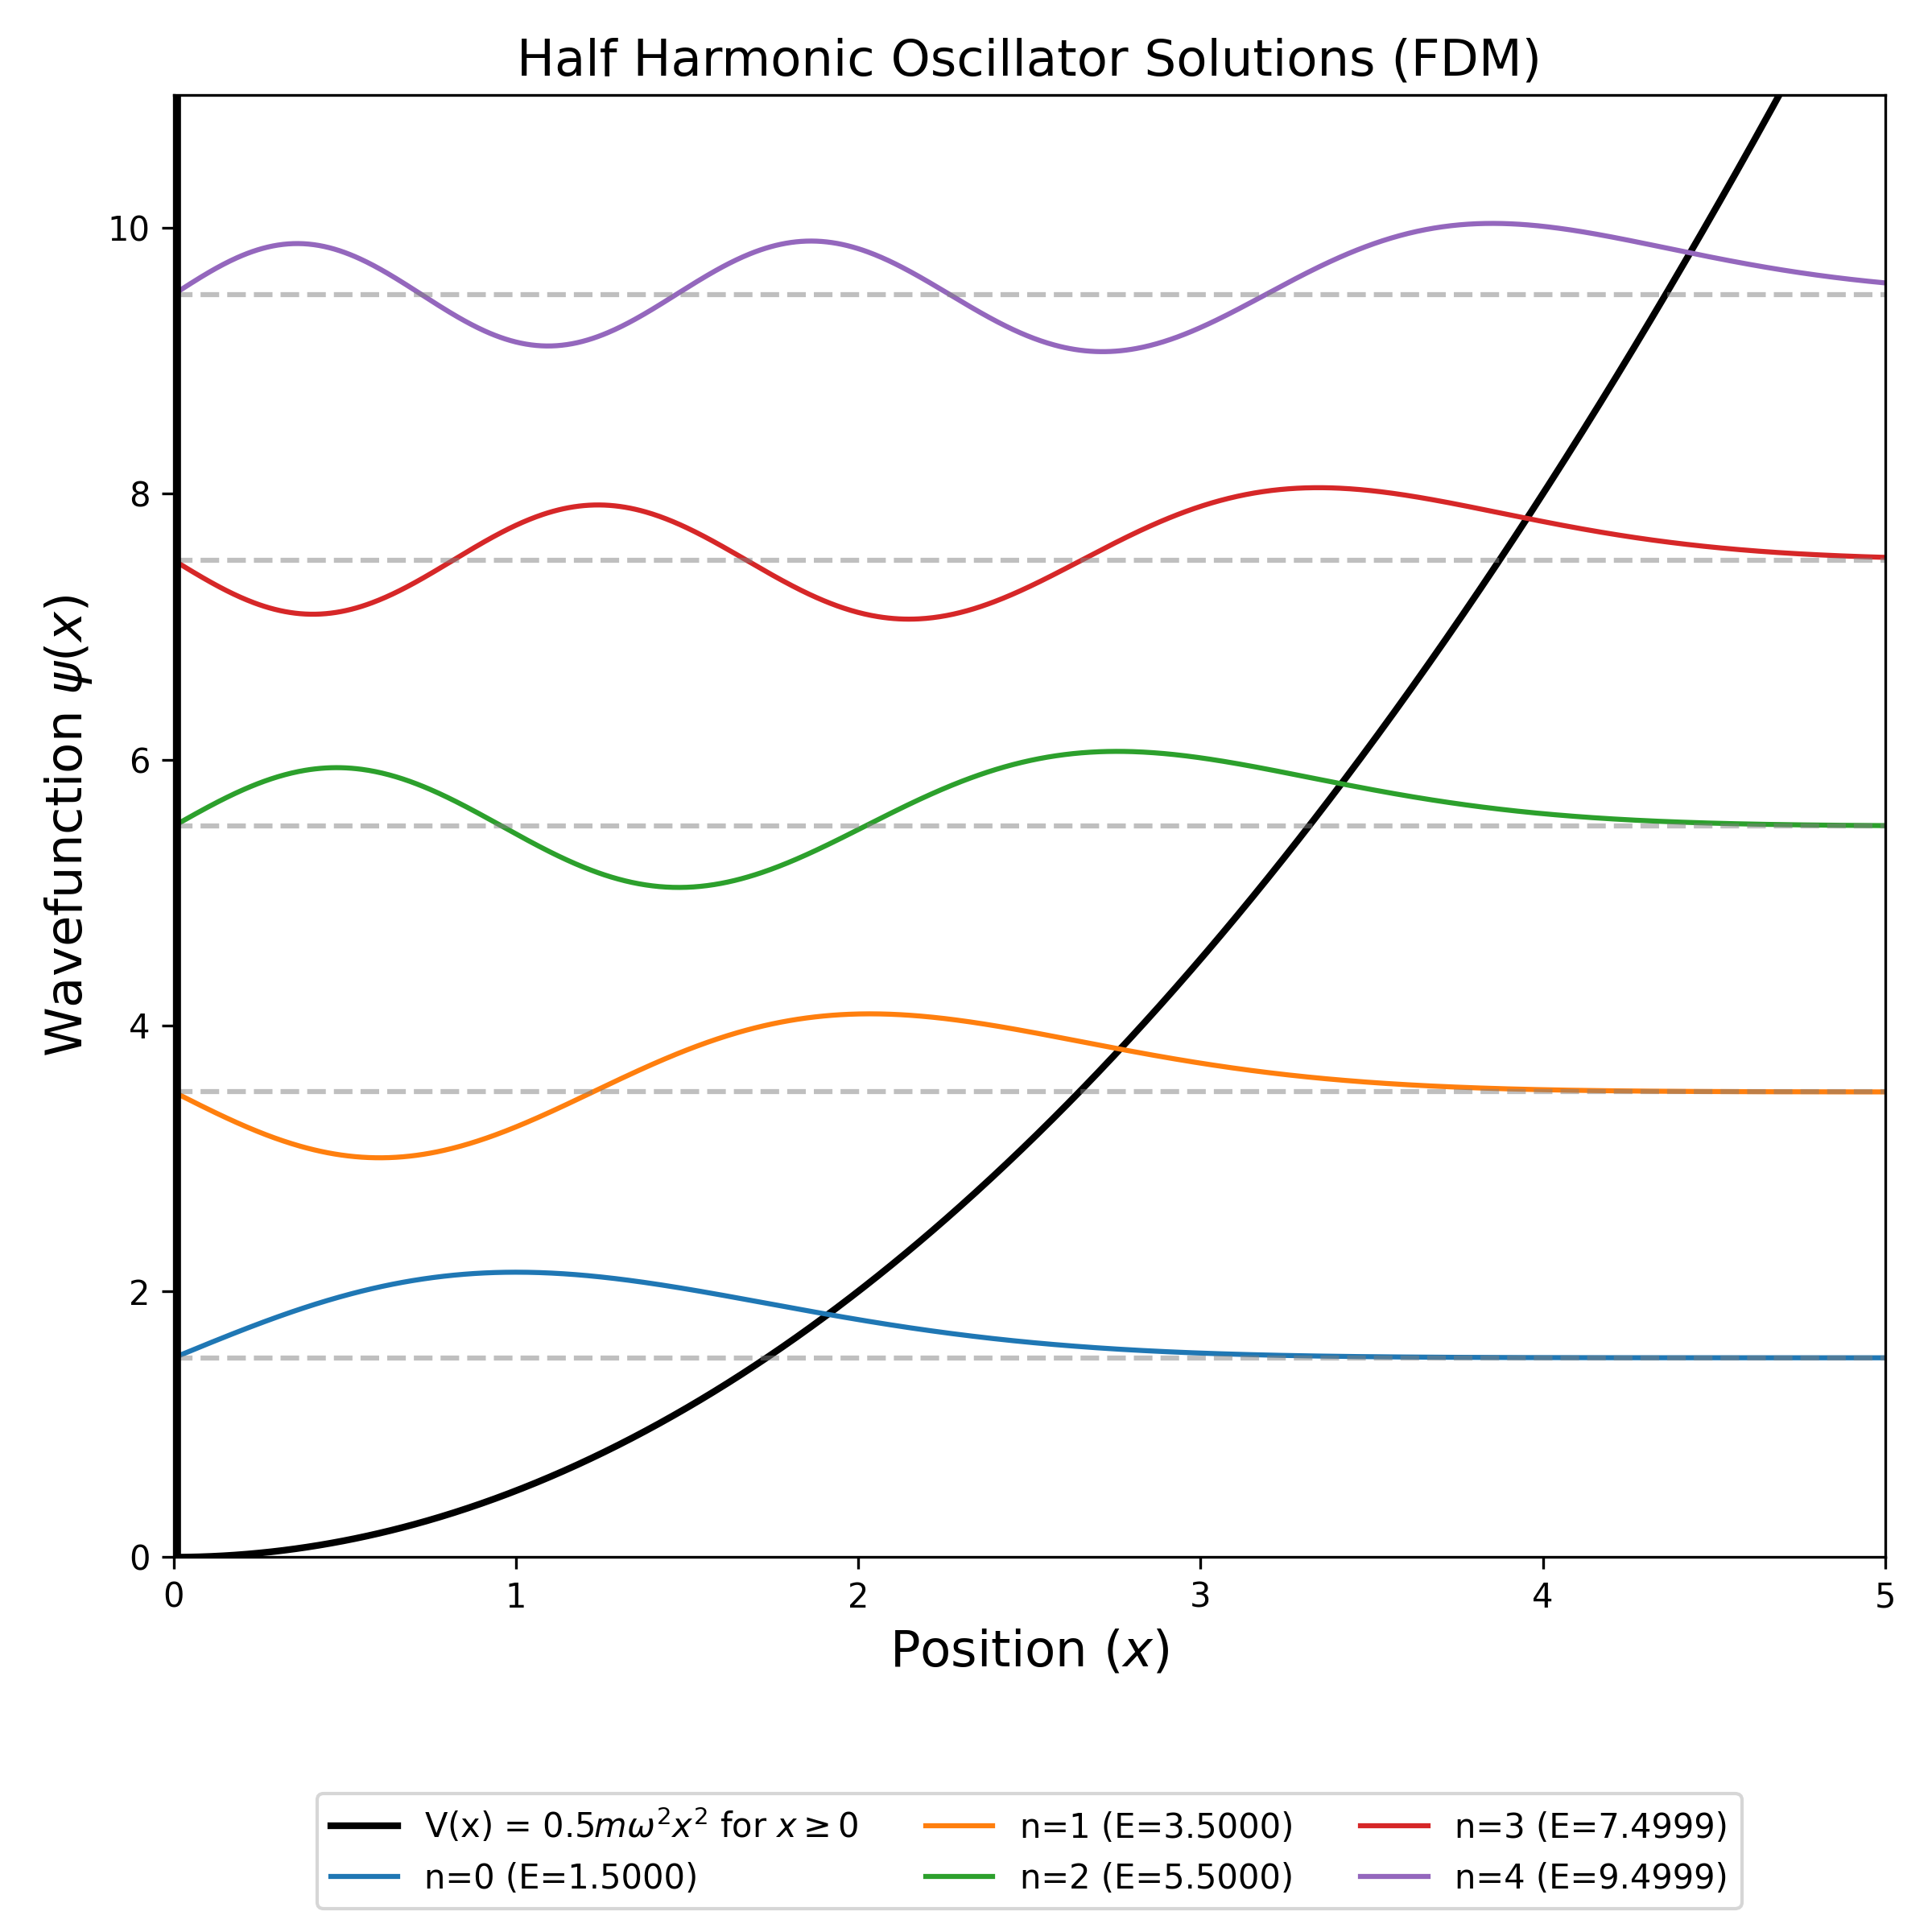
\includegraphics[width=0.8\textwidth]{plots/prob02_half_harmonic.png}
            \label{fig:prob02_wavefunction}
            \end{figure}
            \item {\bf Plot Analysis: } The infinite wall forces $\psi(0) = 0$. Consequently, the valid solutions are exactly the odd-parity wavefunctions of the full harmonic oscillator. The full oscillator's even-parity ground state is destroyed.
        \end{itemize}

        \subsection{Problem 3: One-dimensional Harmonic Potential}
        \begin{itemize}
            \item {\bf Description: } A standard harmonic oscillator.
            \item {\bf Potential: }  $V(x) = \frac{1}{2}m\omega^2 x^2$.
            \item {\bf Code: } \lstinputlisting[style= codestyle]{src/problems/prob03_harmonic_oscillator.f90}
            \item {\bf Output: } \lstinputlisting[style= outputstyle]{output/prob03.txt}
            \item {\bf Plot: }The wavefunctions were visualized using the standard scaling script (defined in Section 2.3) with a visual \texttt{scale\_factor} of 6.0 to prevent overlap between the energy levels.\begin{figure}[H]
            \centering
            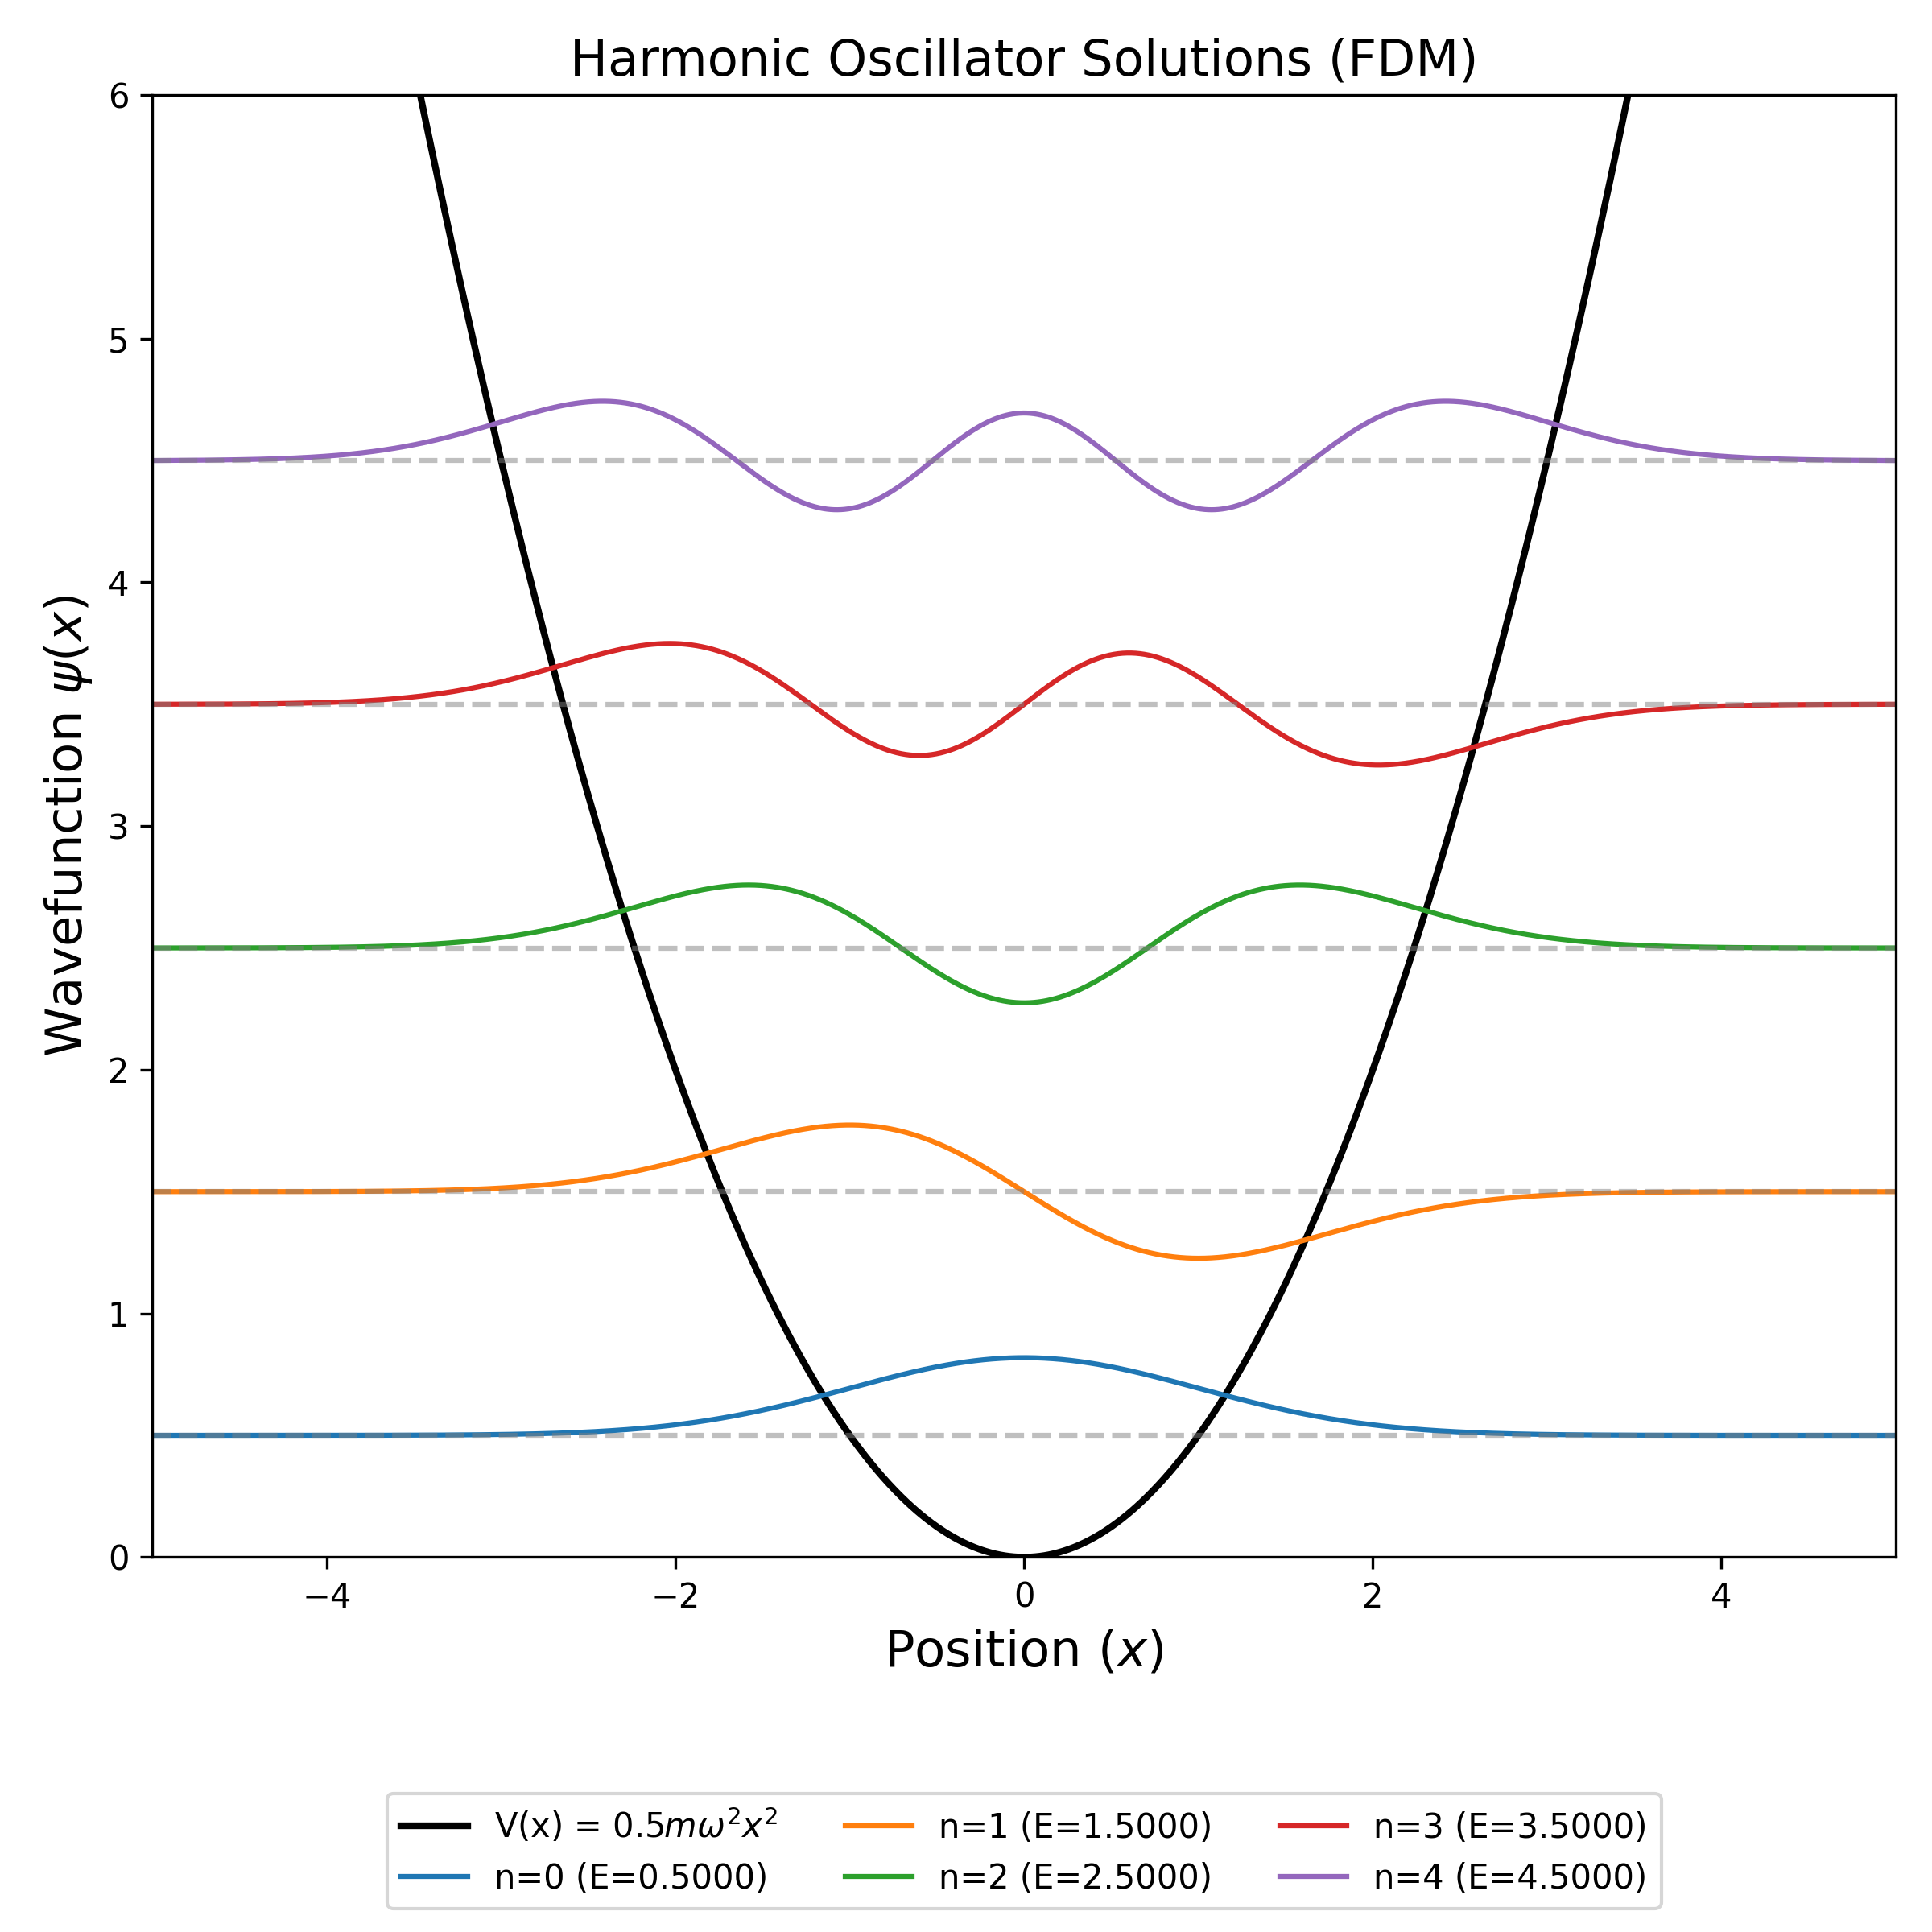
\includegraphics[width=0.8\textwidth]{plots/prob03_harmonic_oscillator.png}
            \label{fig:prob03_wavefunction}
            \end{figure}
            \item {\bf Plot Analysis: } Yields the classic alternating parity states. The ground state is a perfect Gaussian bell curve centered at $x=0$.
        \end{itemize}

        \subsection{Problem 4: Finite Potential Well}
        \begin{itemize}
            \item {\bf Description: } A well with a finite depth $V_0$, allowing the particle to escape if $E > V_0$.
            \item {\bf Potential: }  $V(x) = 0$ when $-L \le x \le +L$, and $V_0$ elsewhere.
            \item {\bf Code: } \lstinputlisting[style= codestyle]{src/problems/prob04_finite_square_well.f90}
            \item {\bf Output: } \lstinputlisting[style= outputstyle]{output/prob04.txt}
            \item {\bf Plot: }The wavefunctions were visualized using the standard scaling script (defined in Section 2.3) with a visual \texttt{scale\_factor} of 25.0 to prevent overlap between the energy levels.\begin{figure}[H]
            \centering
            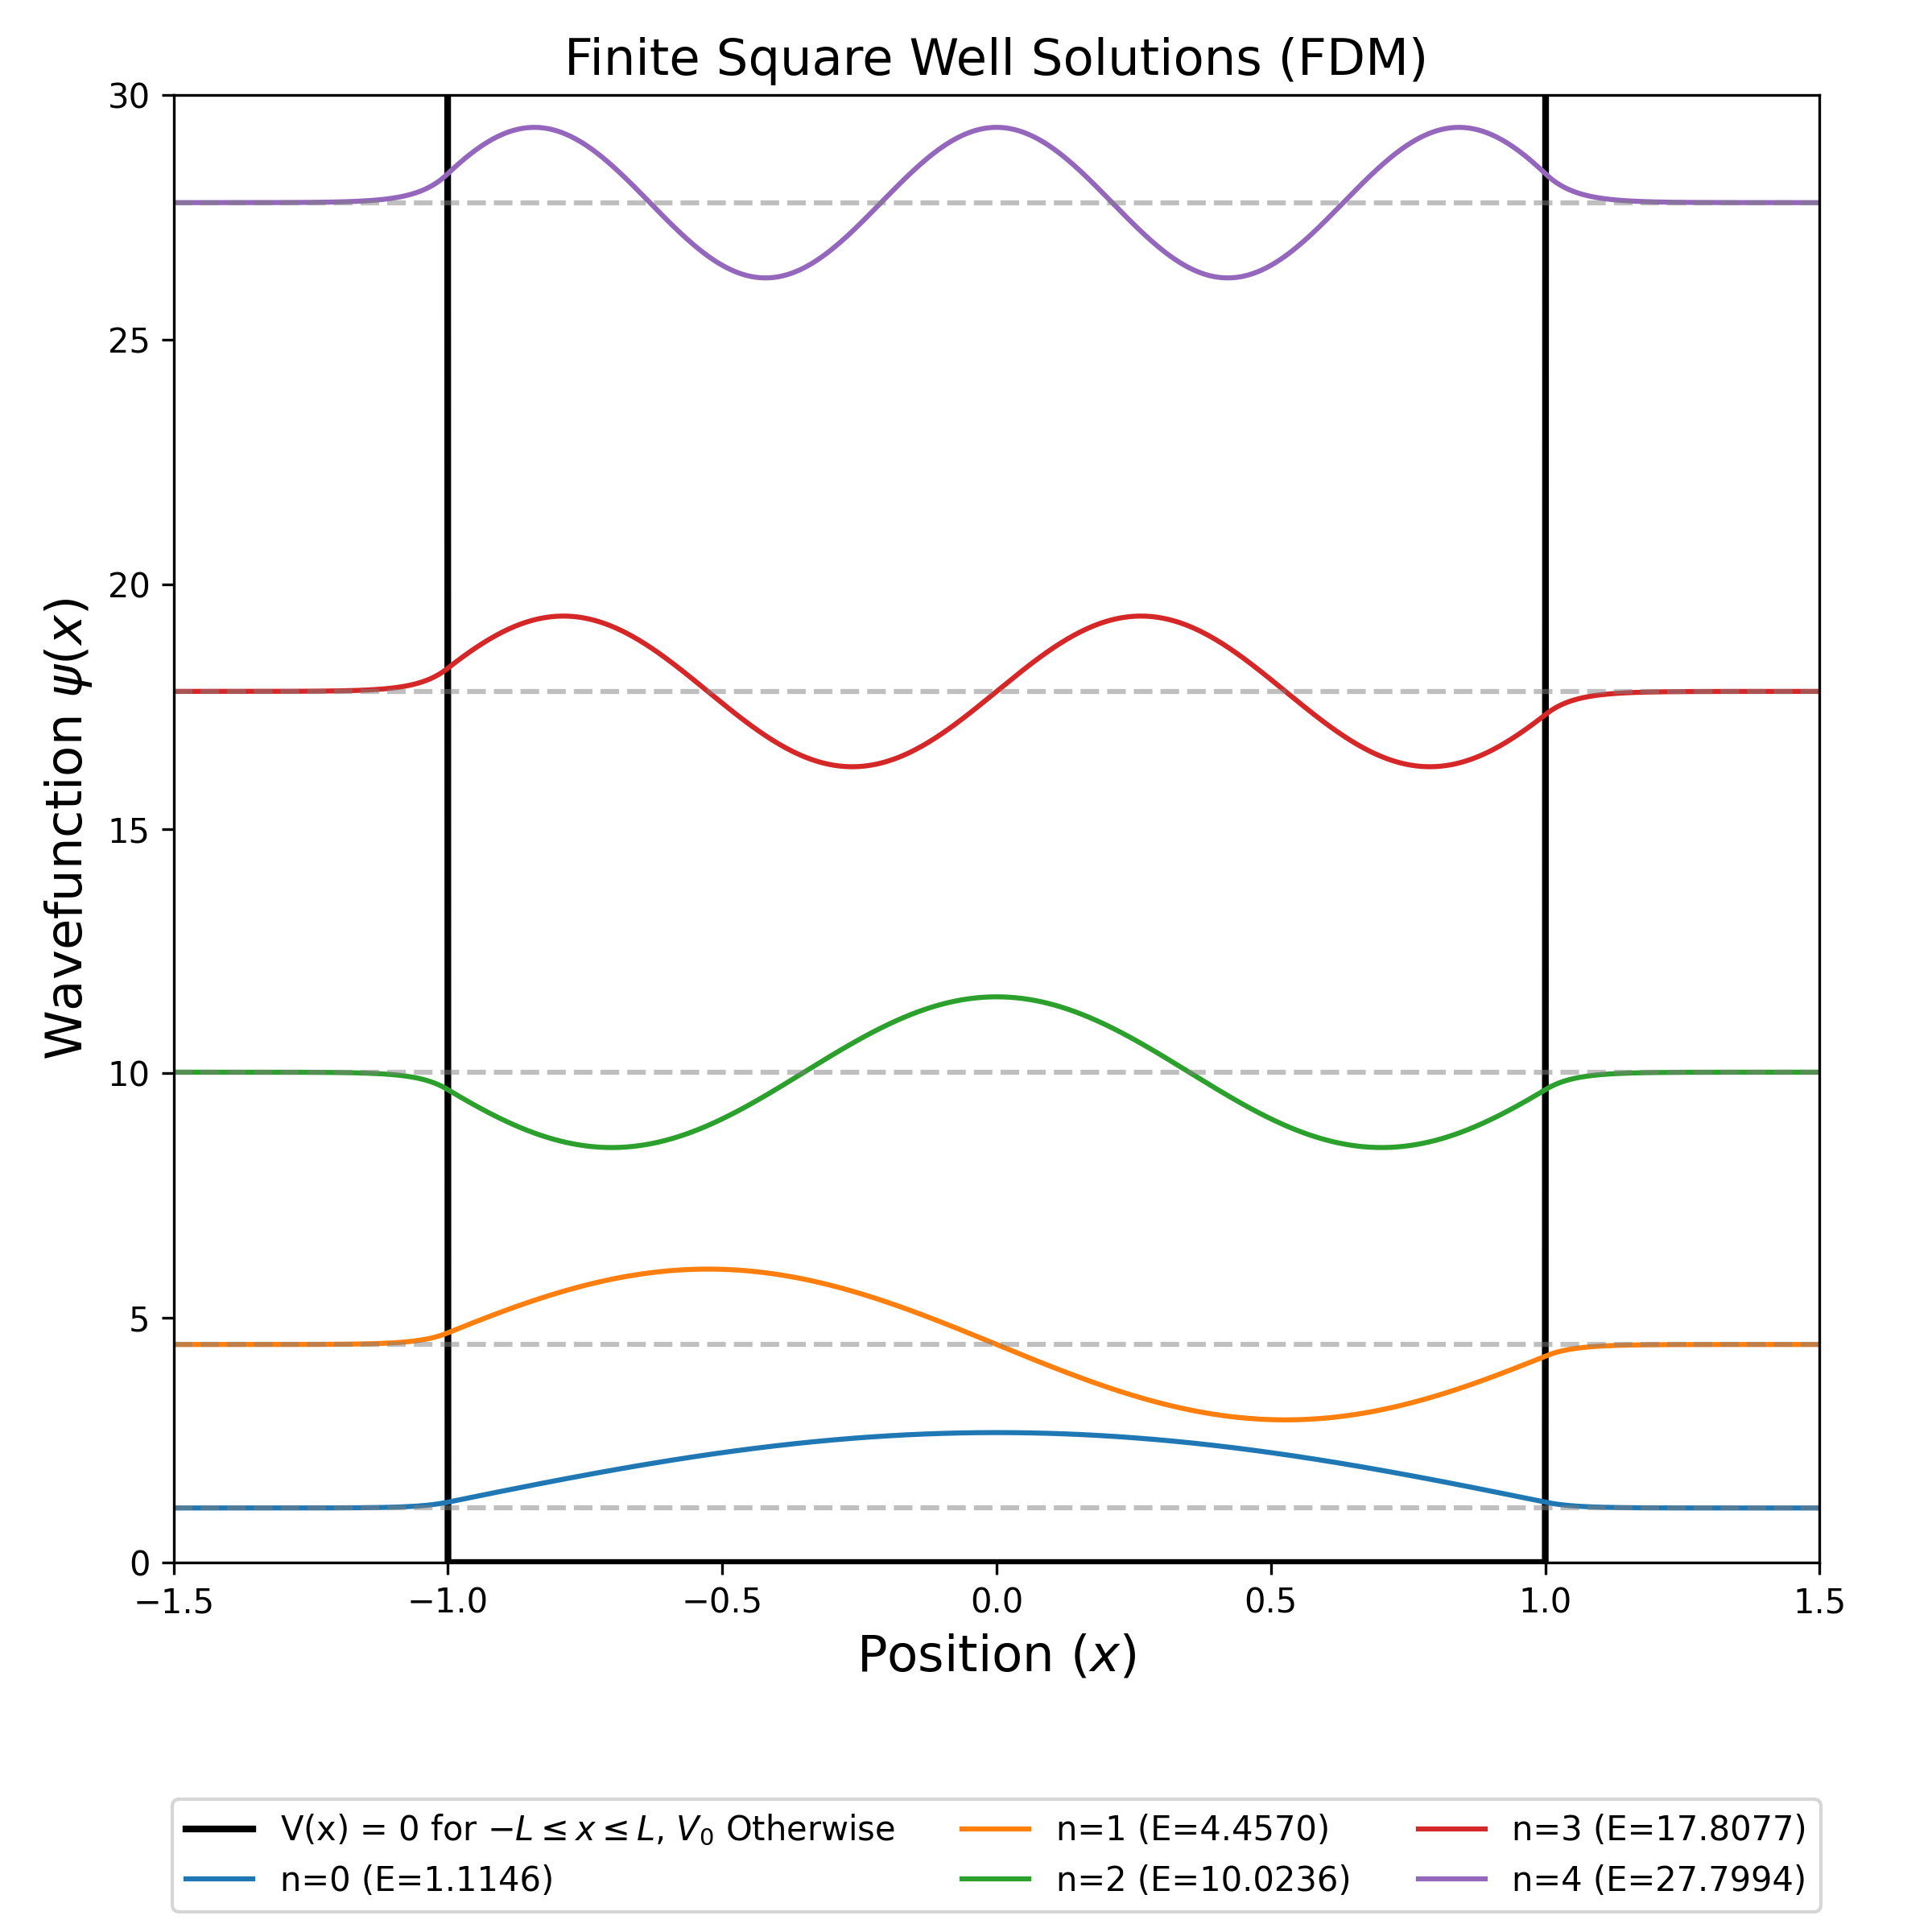
\includegraphics[width=0.8\textwidth]{plots/prob04_finite_square_well.png}
            \label{fig:prob04_wavefunction}
            \end{figure}
            \item {\bf Plot Analysis: } The wavefunctions exhibit sinusoidal behavior inside the well but transition to exponential decay in the classically forbidden regions ($|x| > L$). This demonstrates quantum penetration.
        \end{itemize}

        \subsection{Problem 5: Parabolic Base Infinite Well} 
        \begin{itemize}
            \item {\bf Description: } An infinite well where the floor curves upwards as a parabola.
            \item {\bf Potential: }  $V(x) = \frac{V_0}{L^2}x^2$ for $0 \le x \le L$, and $\infty$ elsewhere.
            \item {\bf Code: } \lstinputlisting[style= codestyle]{src/problems/prob05_parabolic_base.f90}
            \item {\bf Output: } \lstinputlisting[style= outputstyle]{output/prob05.txt}
            \item {\bf Plot: }The wavefunctions were visualized using the standard scaling script (defined in Section 2.3) with a visual \texttt{scale\_factor} of 1000.0 to prevent overlap between the energy levels.\begin{figure}[H]
            \centering
            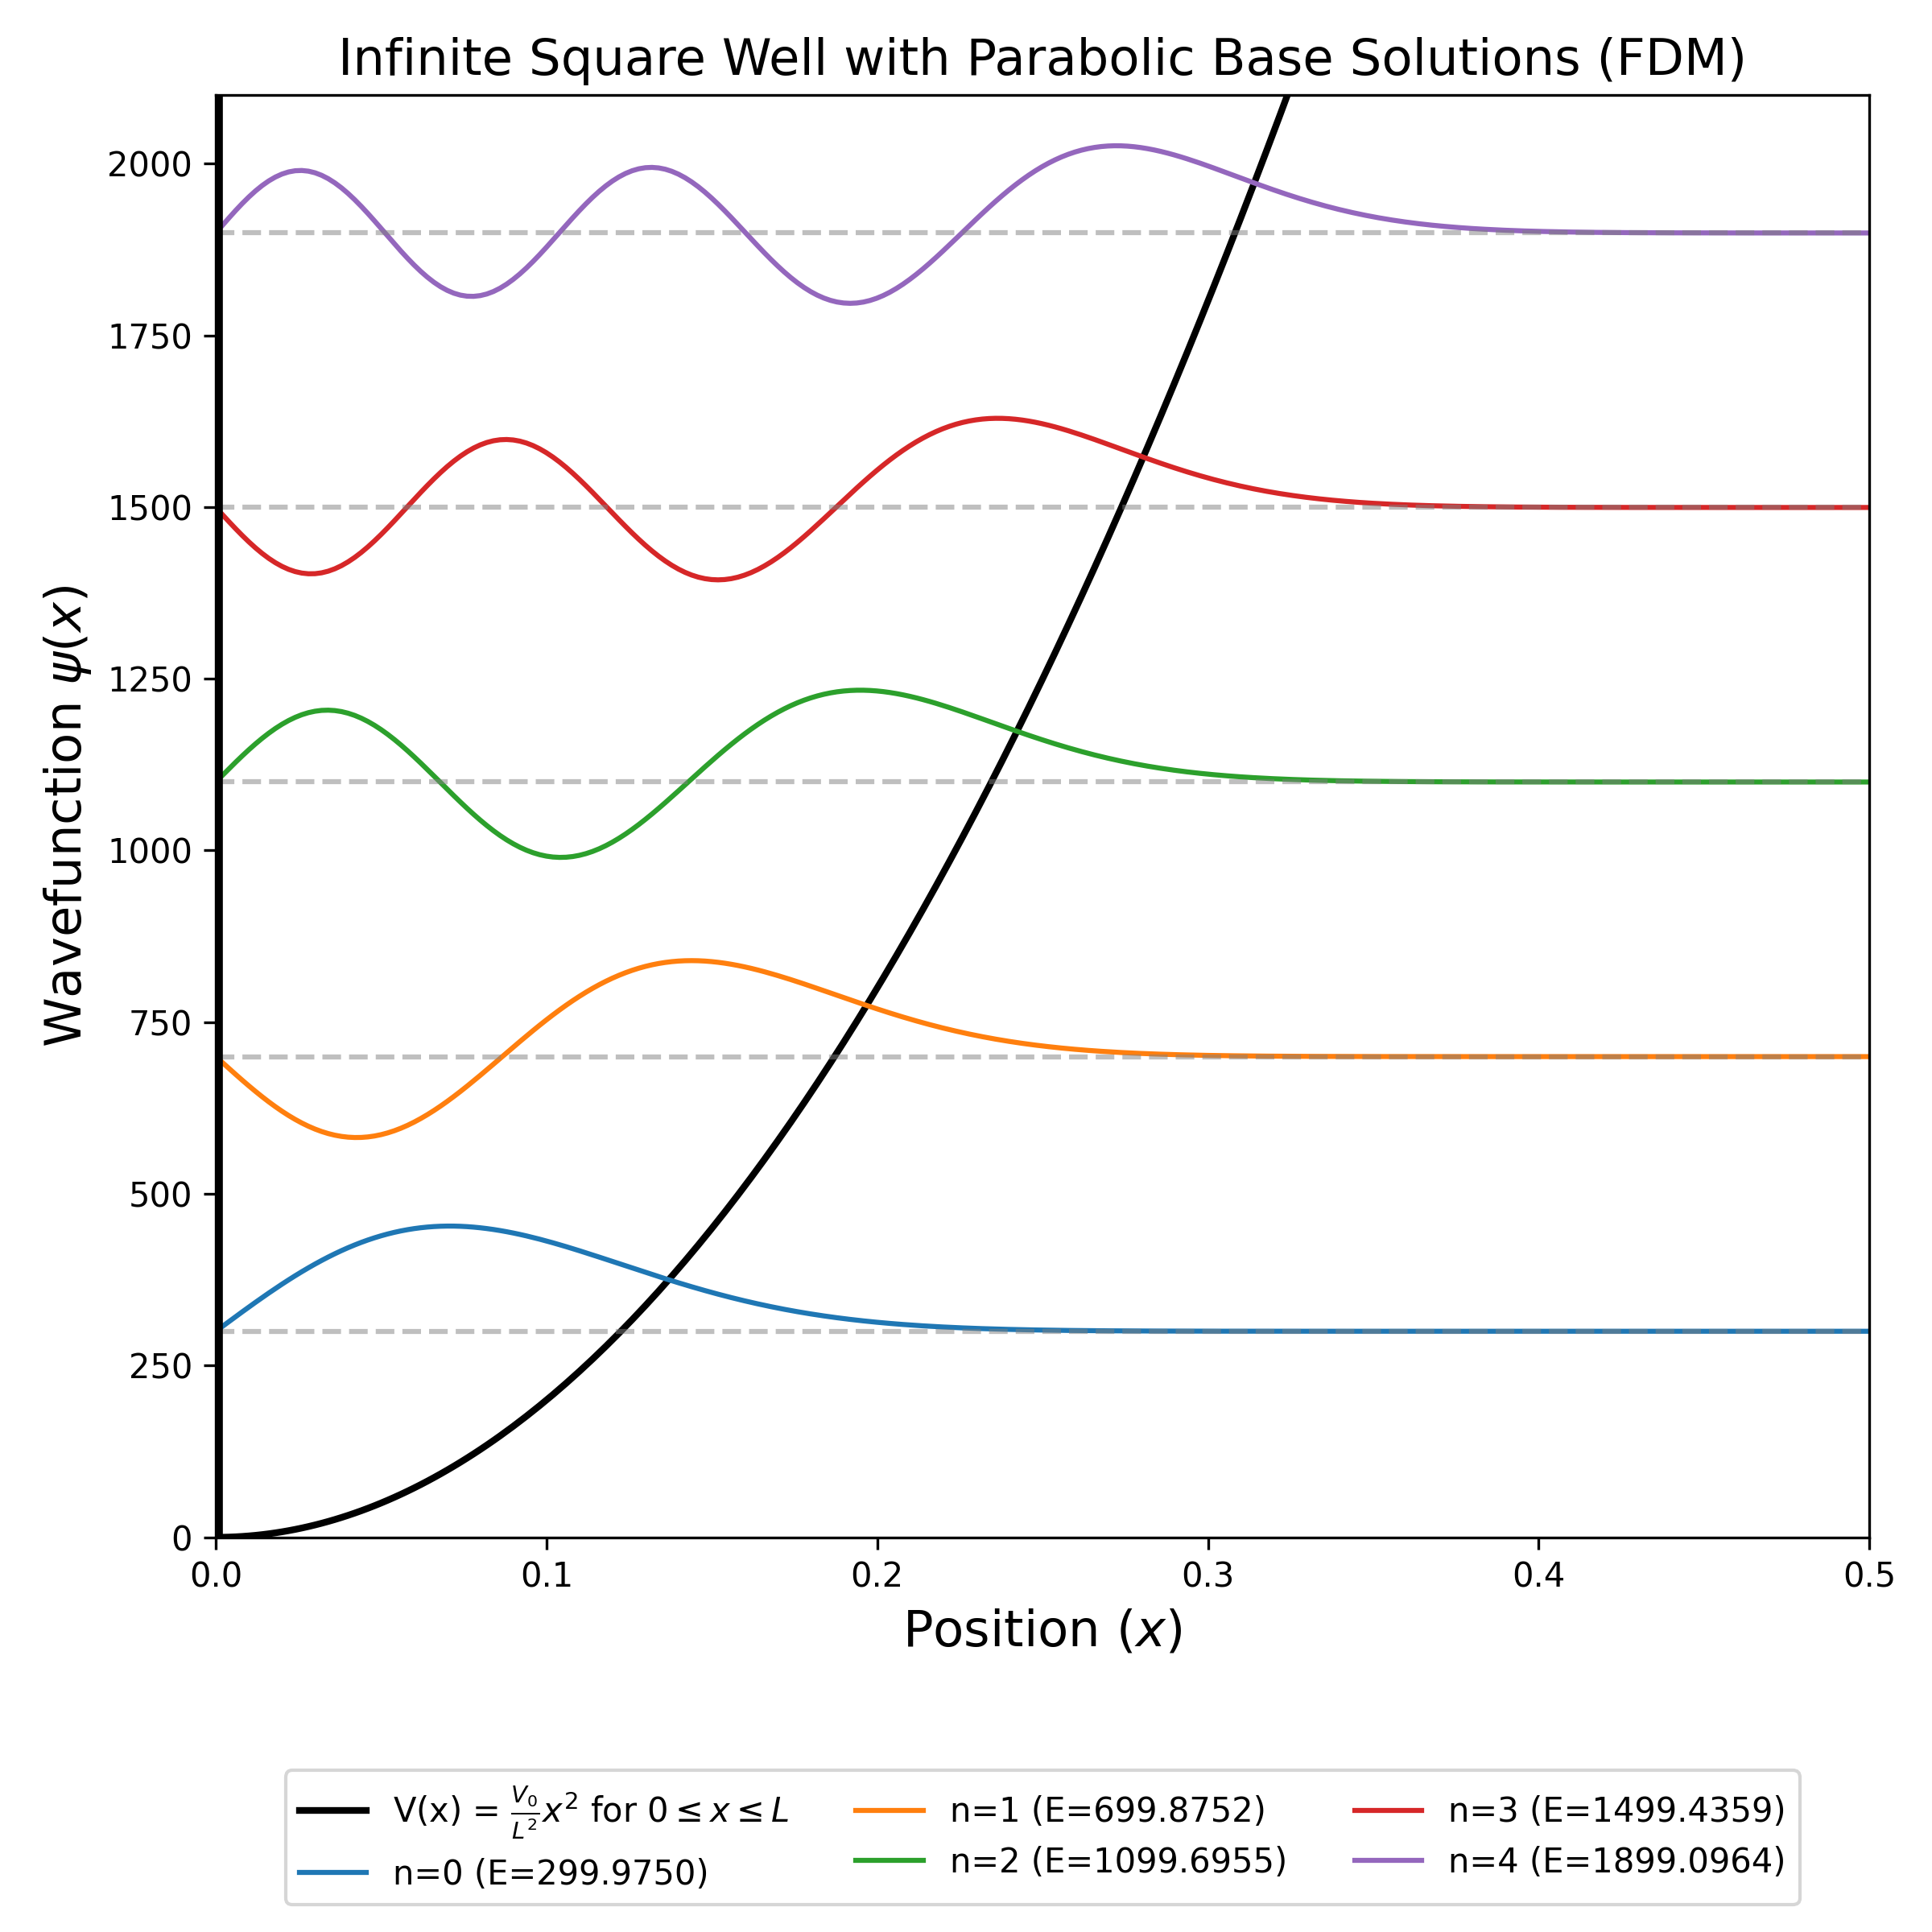
\includegraphics[width=0.8\textwidth]{plots/prob05_infinite_square_well_parabolic_base_.png}
            \label{fig:prob05_wavefunction}
            \end{figure}
            \item {\bf Plot Analysis: } Combines features of the harmonic oscillator and the infinite well. The wavefunctions are squeezed inward by the parabolic floor but forcefully truncated at the infinite boundaries.
        \end{itemize}

        \subsection{Problem 6: Modulo \texorpdfstring{$x$}{x} Potential} 
        \begin{itemize}
            \item {\bf Description: } A V-shaped linear potential well.
            \item {\bf Potential: } $V(x) = |x|$.
            \item {\bf Code: } \lstinputlisting[style= codestyle]{src/problems/prob06_mod_x.f90}
            \item {\bf Output: } \lstinputlisting[style= outputstyle]{output/prob06.txt}
            \item {\bf Plot: }The wavefunctions were visualized using the standard scaling script (defined in Section 2.3) with a visual \texttt{scale\_factor} of 6.0 to prevent overlap between the energy levels.\begin{figure}[H]
            \centering
            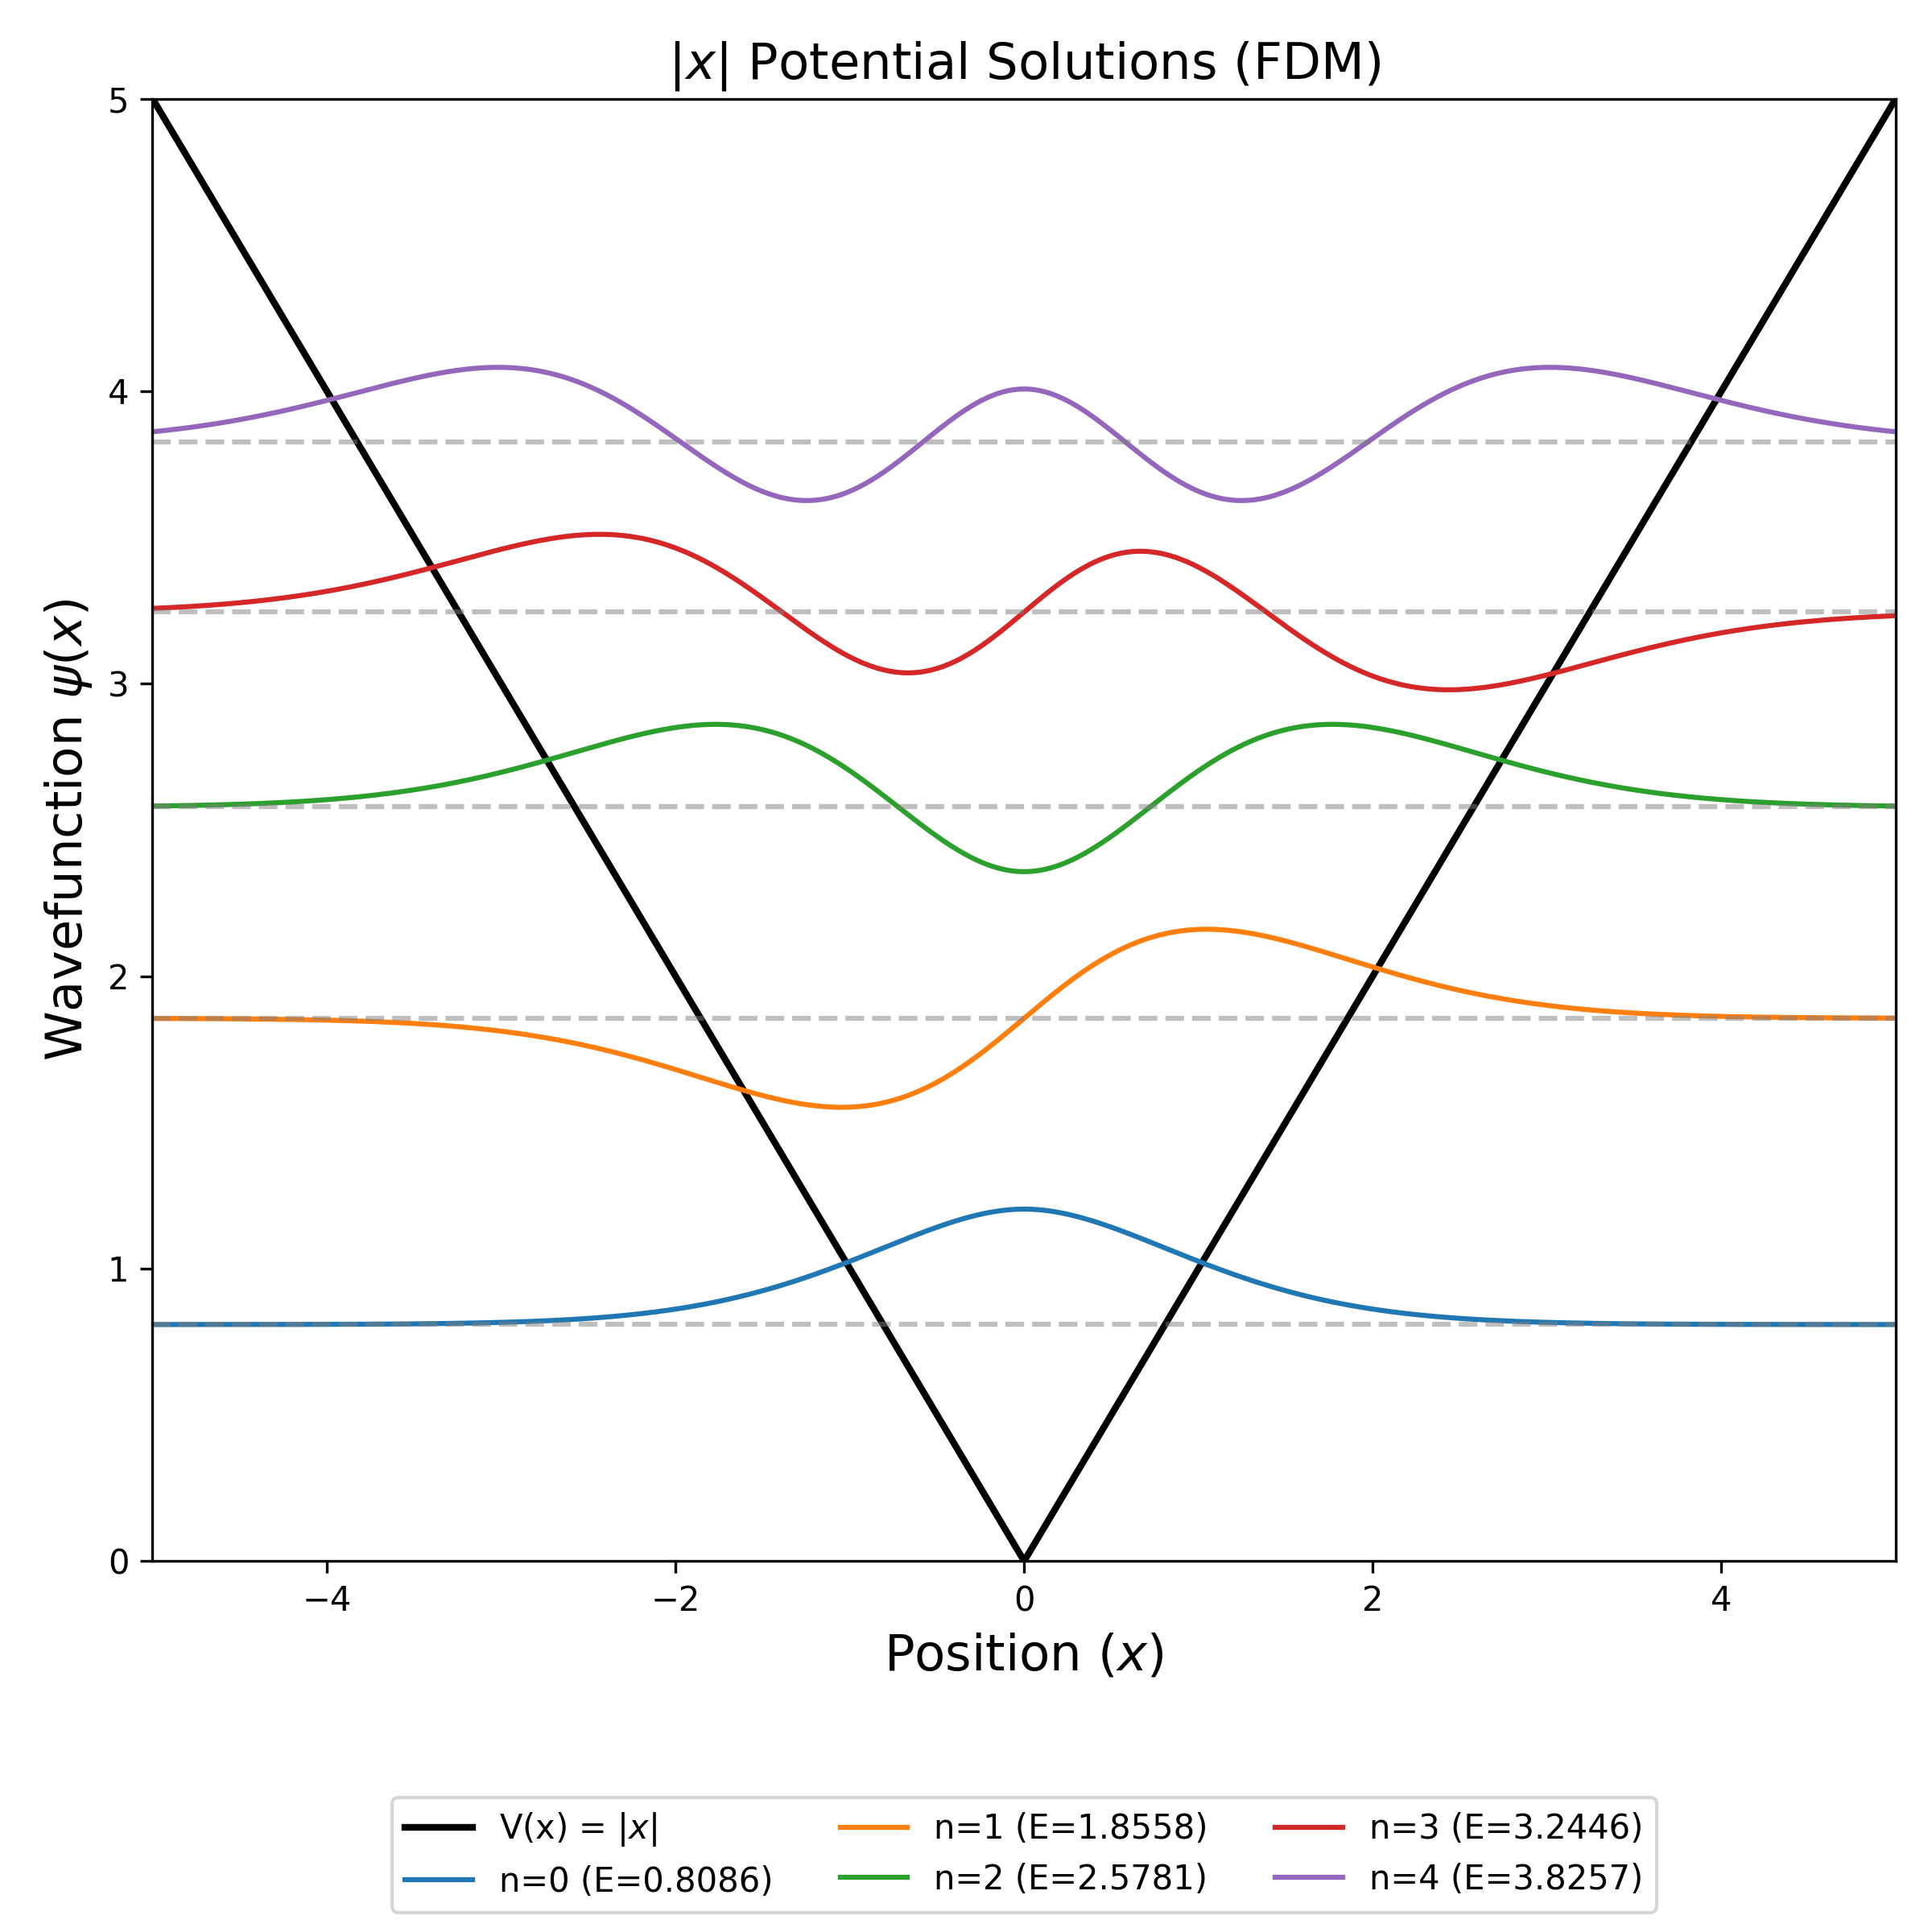
\includegraphics[width=0.8\textwidth]{plots/prob06_mod_x.png}
            \label{fig:prob06_wavefunction}
            \end{figure}
            \item {\bf Plot Analysis: } The states are tightly bound at the bottom of the "V". Because the potential rises linearly rather than quadratically, the energy levels are spaced more closely together than in the harmonic oscillator.
        \end{itemize}

        \subsection{Problem 7: Modulo \texorpdfstring{$x^3$}{x} Potential} 
        \begin{itemize}
            \item {\bf Description: } A steep, non-harmonic symmetric well.
            \item {\bf Potential: } $V(x) = |x^3|$.
            \item {\bf Code: } \lstinputlisting[style= codestyle]{src/problems/prob07_mod_x_cube.f90}
            \item {\bf Output: } \lstinputlisting[style= outputstyle]{output/prob07.txt}
            \item {\bf Plot: }The wavefunctions were visualized using the standard scaling script (defined in Section 2.3) with a visual \texttt{scale\_factor} of 15.0 to prevent overlap between the energy levels.\begin{figure}[H]
            \centering
            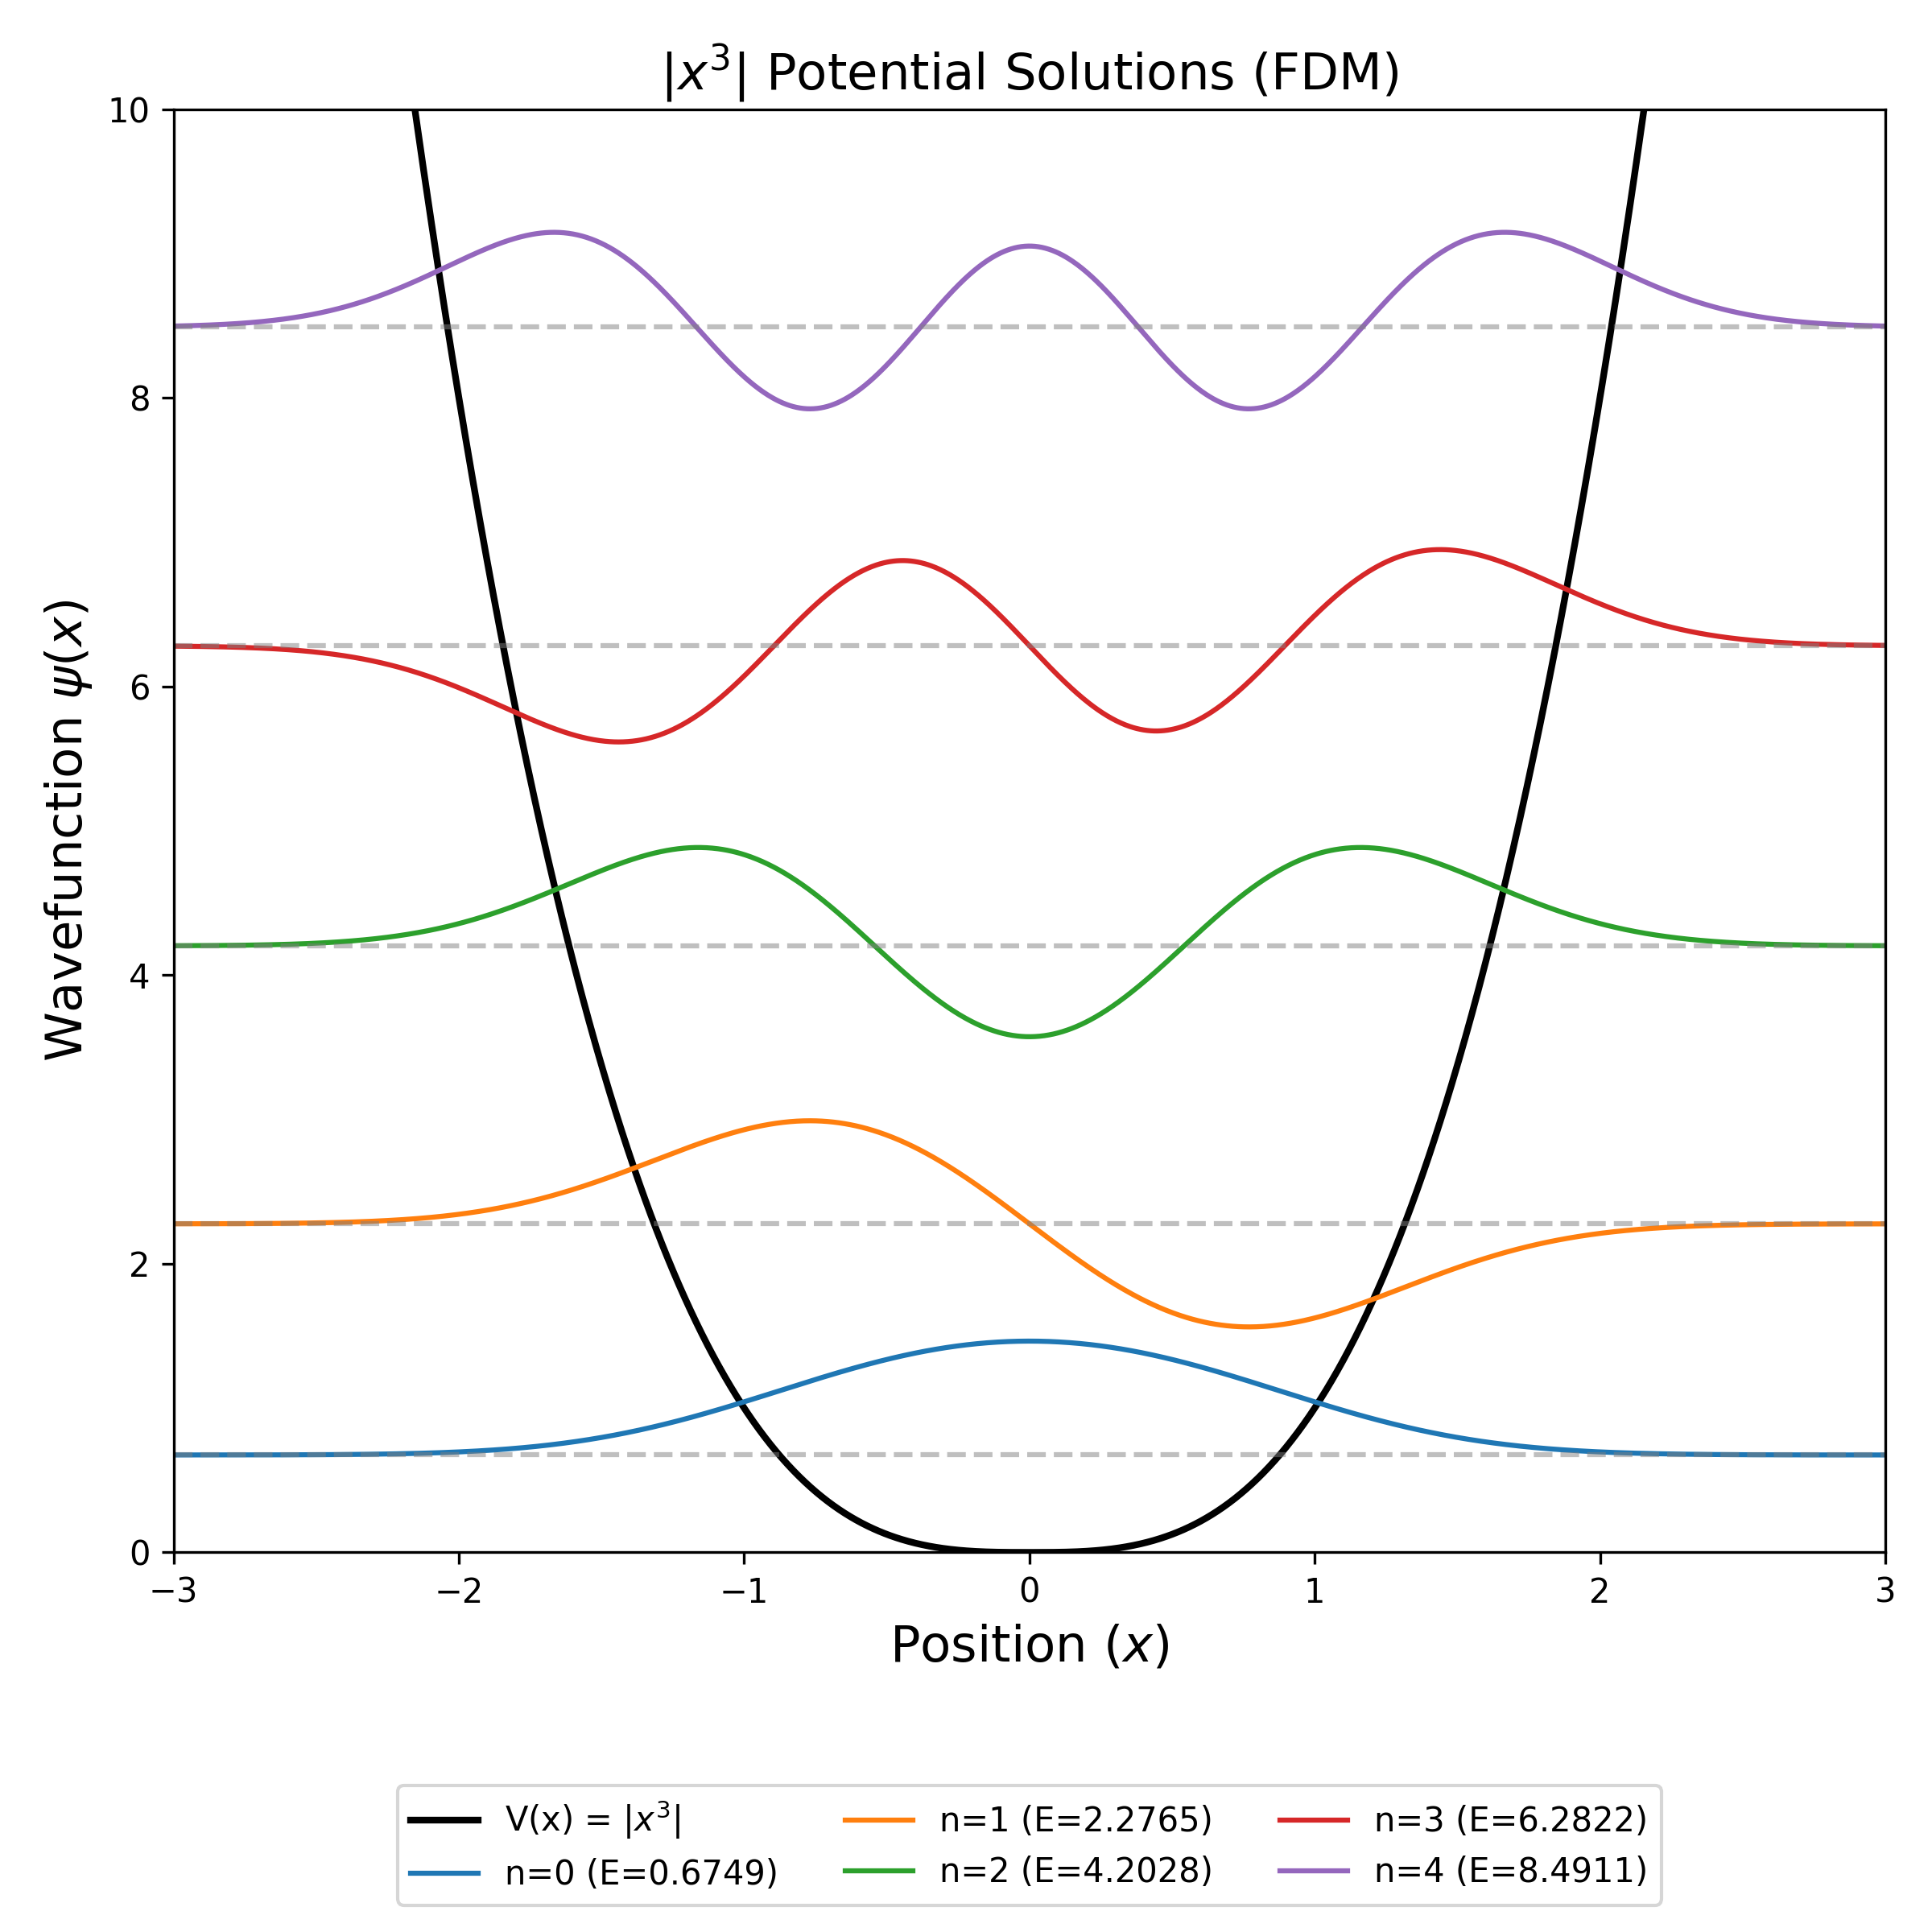
\includegraphics[width=0.8\textwidth]{plots/prob07_mod_x_cube.png}
            \label{fig:prob07_wavefunction}
            \end{figure}
            \item {\bf Plot Analysis: } The potential walls rise much faster than a parabola. This tighter spatial confinement leads to energy levels that spread further apart as $n$ increases, contrasting with the evenly spaced levels of the harmonic oscillator.
        \end{itemize}

        \subsection{Problem 8: Quartic Potential} 
        \begin{itemize}
            \item {\bf Description: } A symmetric well with walls that rise as $x^4$.
            \item {\bf Potential: } $V(x) = x^4$.
            \item {\bf Code: } \lstinputlisting[style= codestyle]{src/problems/prob08_quartic_potential.f90}
            \item {\bf Output: } \lstinputlisting[style= outputstyle]{output/prob08.txt}
            \item {\bf Plot: }The wavefunctions were visualized using the standard scaling script (defined in Section 2.3) with a visual \texttt{scale\_factor} of 15.0 to prevent overlap between the energy levels.\begin{figure}[H]
            \centering
            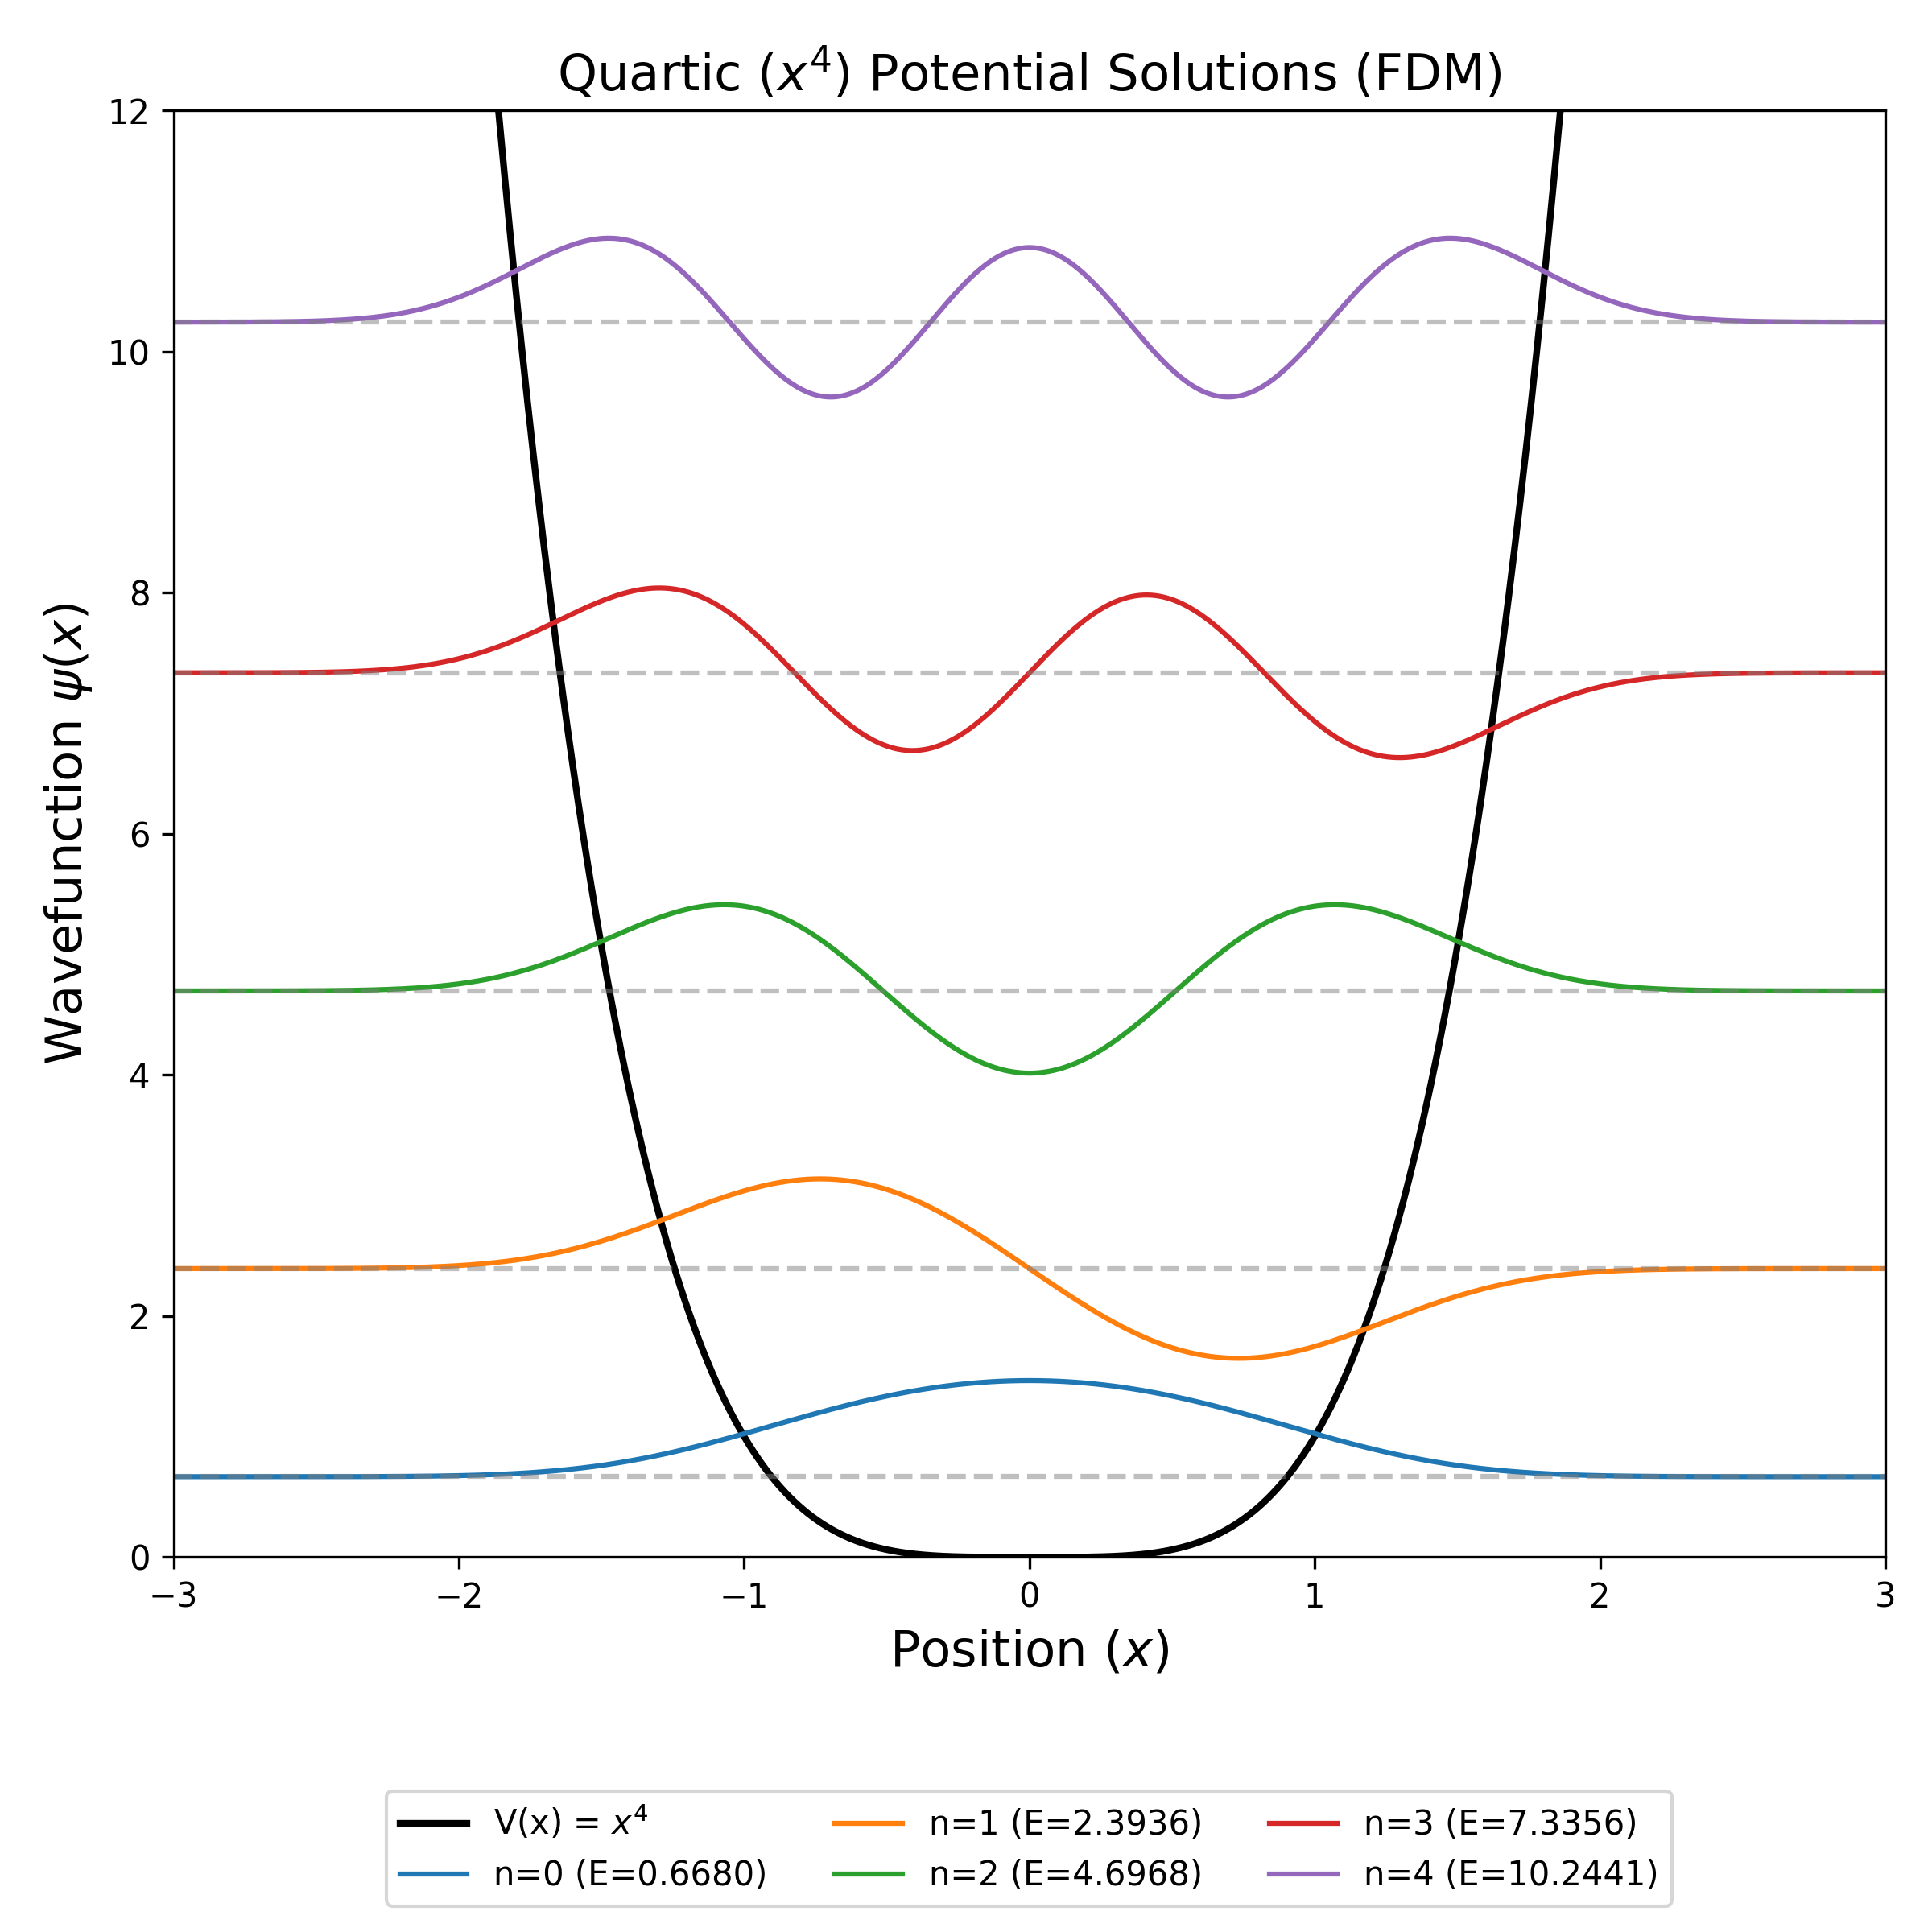
\includegraphics[width=0.8\textwidth]{plots/prob08_quartic_potential.png}
            \label{fig:prob08_wavefunction}
            \end{figure}
            \item {\bf Plot Analysis: } Extremely flat at the bottom but incredibly steep at the edges. The wavefunctions near the ground state spread out over the flat bottom, while higher states are abruptly reflected by the steep quartic walls.
        \end{itemize}

        \subsection{Problem 9: Quadratic-Quartic Potential} 
        \begin{itemize}
            \item {\bf Description: } An anharmonic oscillator combining both $x^2$ and $x^4$ terms.
            \item {\bf Potential: } $V(x) = x^2 + x^4$.
            \item {\bf Code: } \lstinputlisting[style= codestyle]{src/problems/prob09_quartic_quadratic.f90}
            \item {\bf Output: } \lstinputlisting[style= outputstyle]{output/prob09.txt}
            \item {\bf Plot: }The wavefunctions were visualized using the standard scaling script (defined in Section 2.3) with a visual \texttt{scale\_factor} of 15.0 to prevent overlap between the energy levels.\begin{figure}[H]
            \centering
            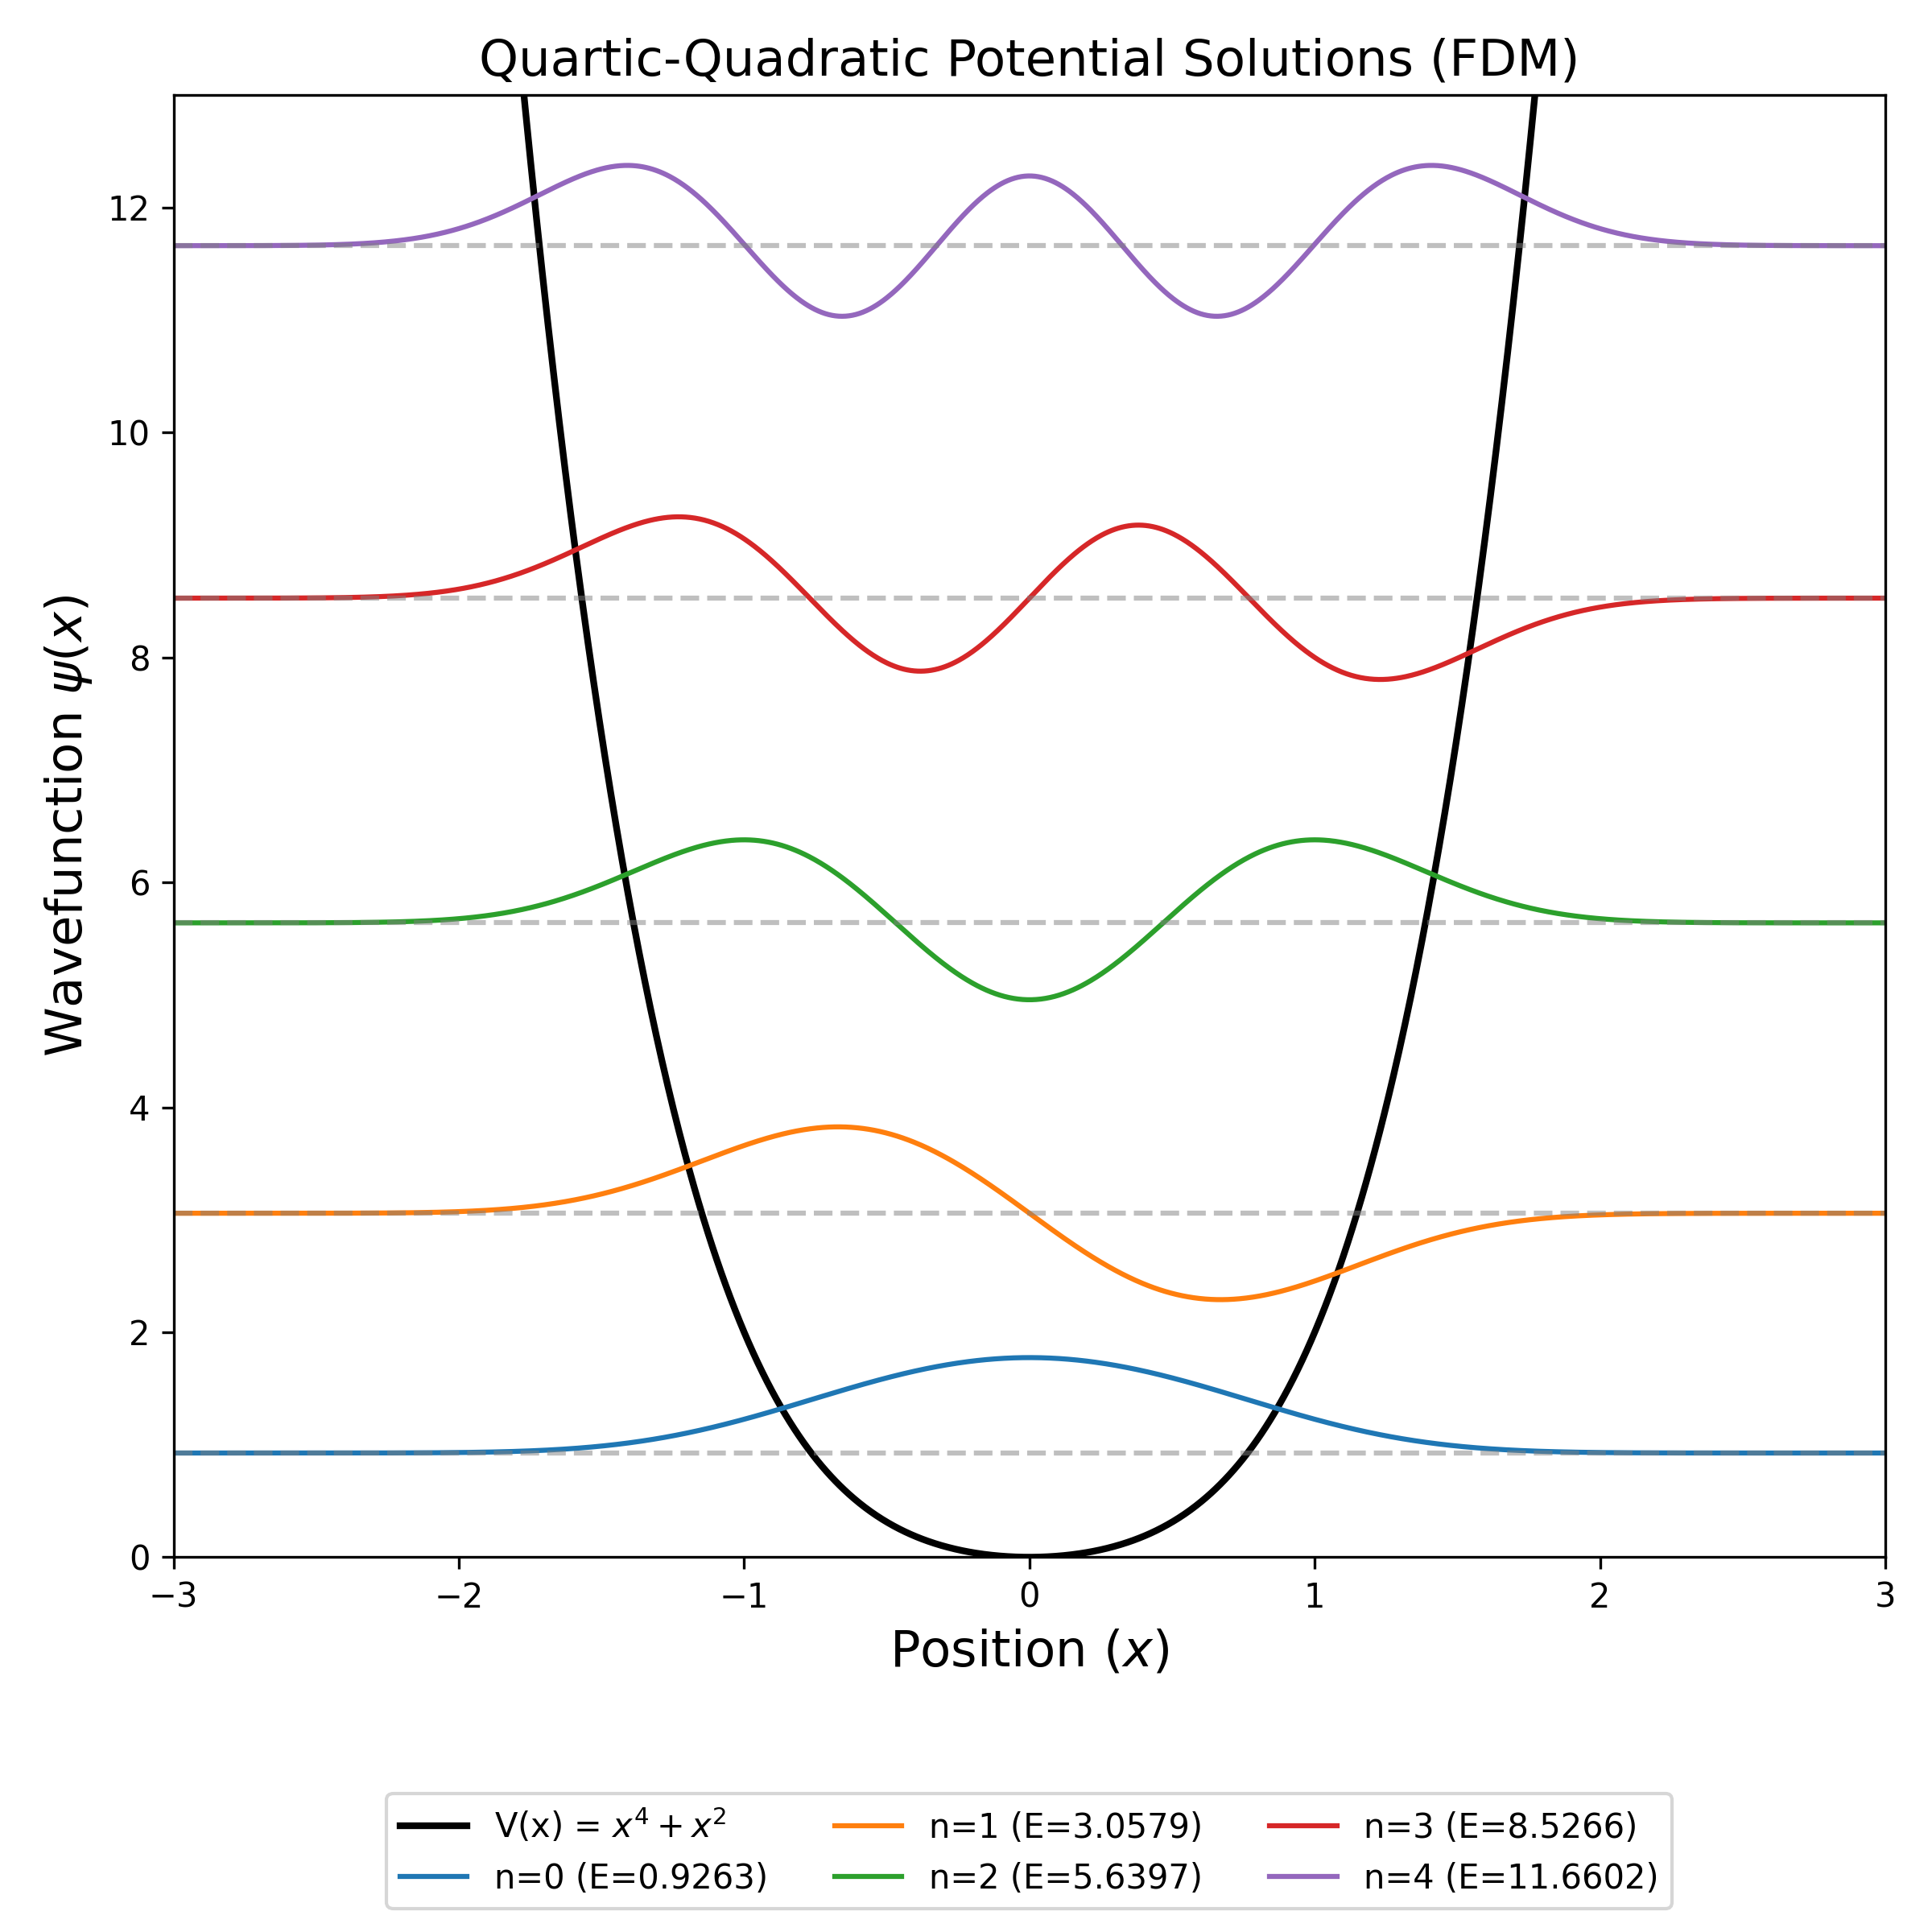
\includegraphics[width=0.8\textwidth]{plots/prob09_quartic_quadratic_potential.png}
            \label{fig:prob09_wavefunction}
            \end{figure}
            \item {\bf Plot Analysis: } The $x^2$ term dominates near the origin, making the ground state resemble a standard harmonic oscillator. For higher energy states, the $x^4$ term dominates, causing the energy gaps to increase rapidly.
        \end{itemize}

        \subsection{Problem 10: Half-Cubic Potential} 
        \begin{itemize}
            \item {\bf Description: }  A cubic well bounded by an infinite wall at the origin.
            \item {\bf Potential: }  $V(x) = x^3$ when $x \ge 0$, and $\infty$ otherwise.
            \item {\bf Code: } \lstinputlisting[style= codestyle]{src/problems/prob10_half_cubic.f90}
            \item {\bf Output: } \lstinputlisting[style= outputstyle]{output/prob10.txt}
            \item {\bf Plot: }The wavefunctions were visualized using the standard scaling script (defined in Section 2.3) with a visual \texttt{scale\_factor} of 30.0 to prevent overlap between the energy levels.\begin{figure}[H]
            \centering
            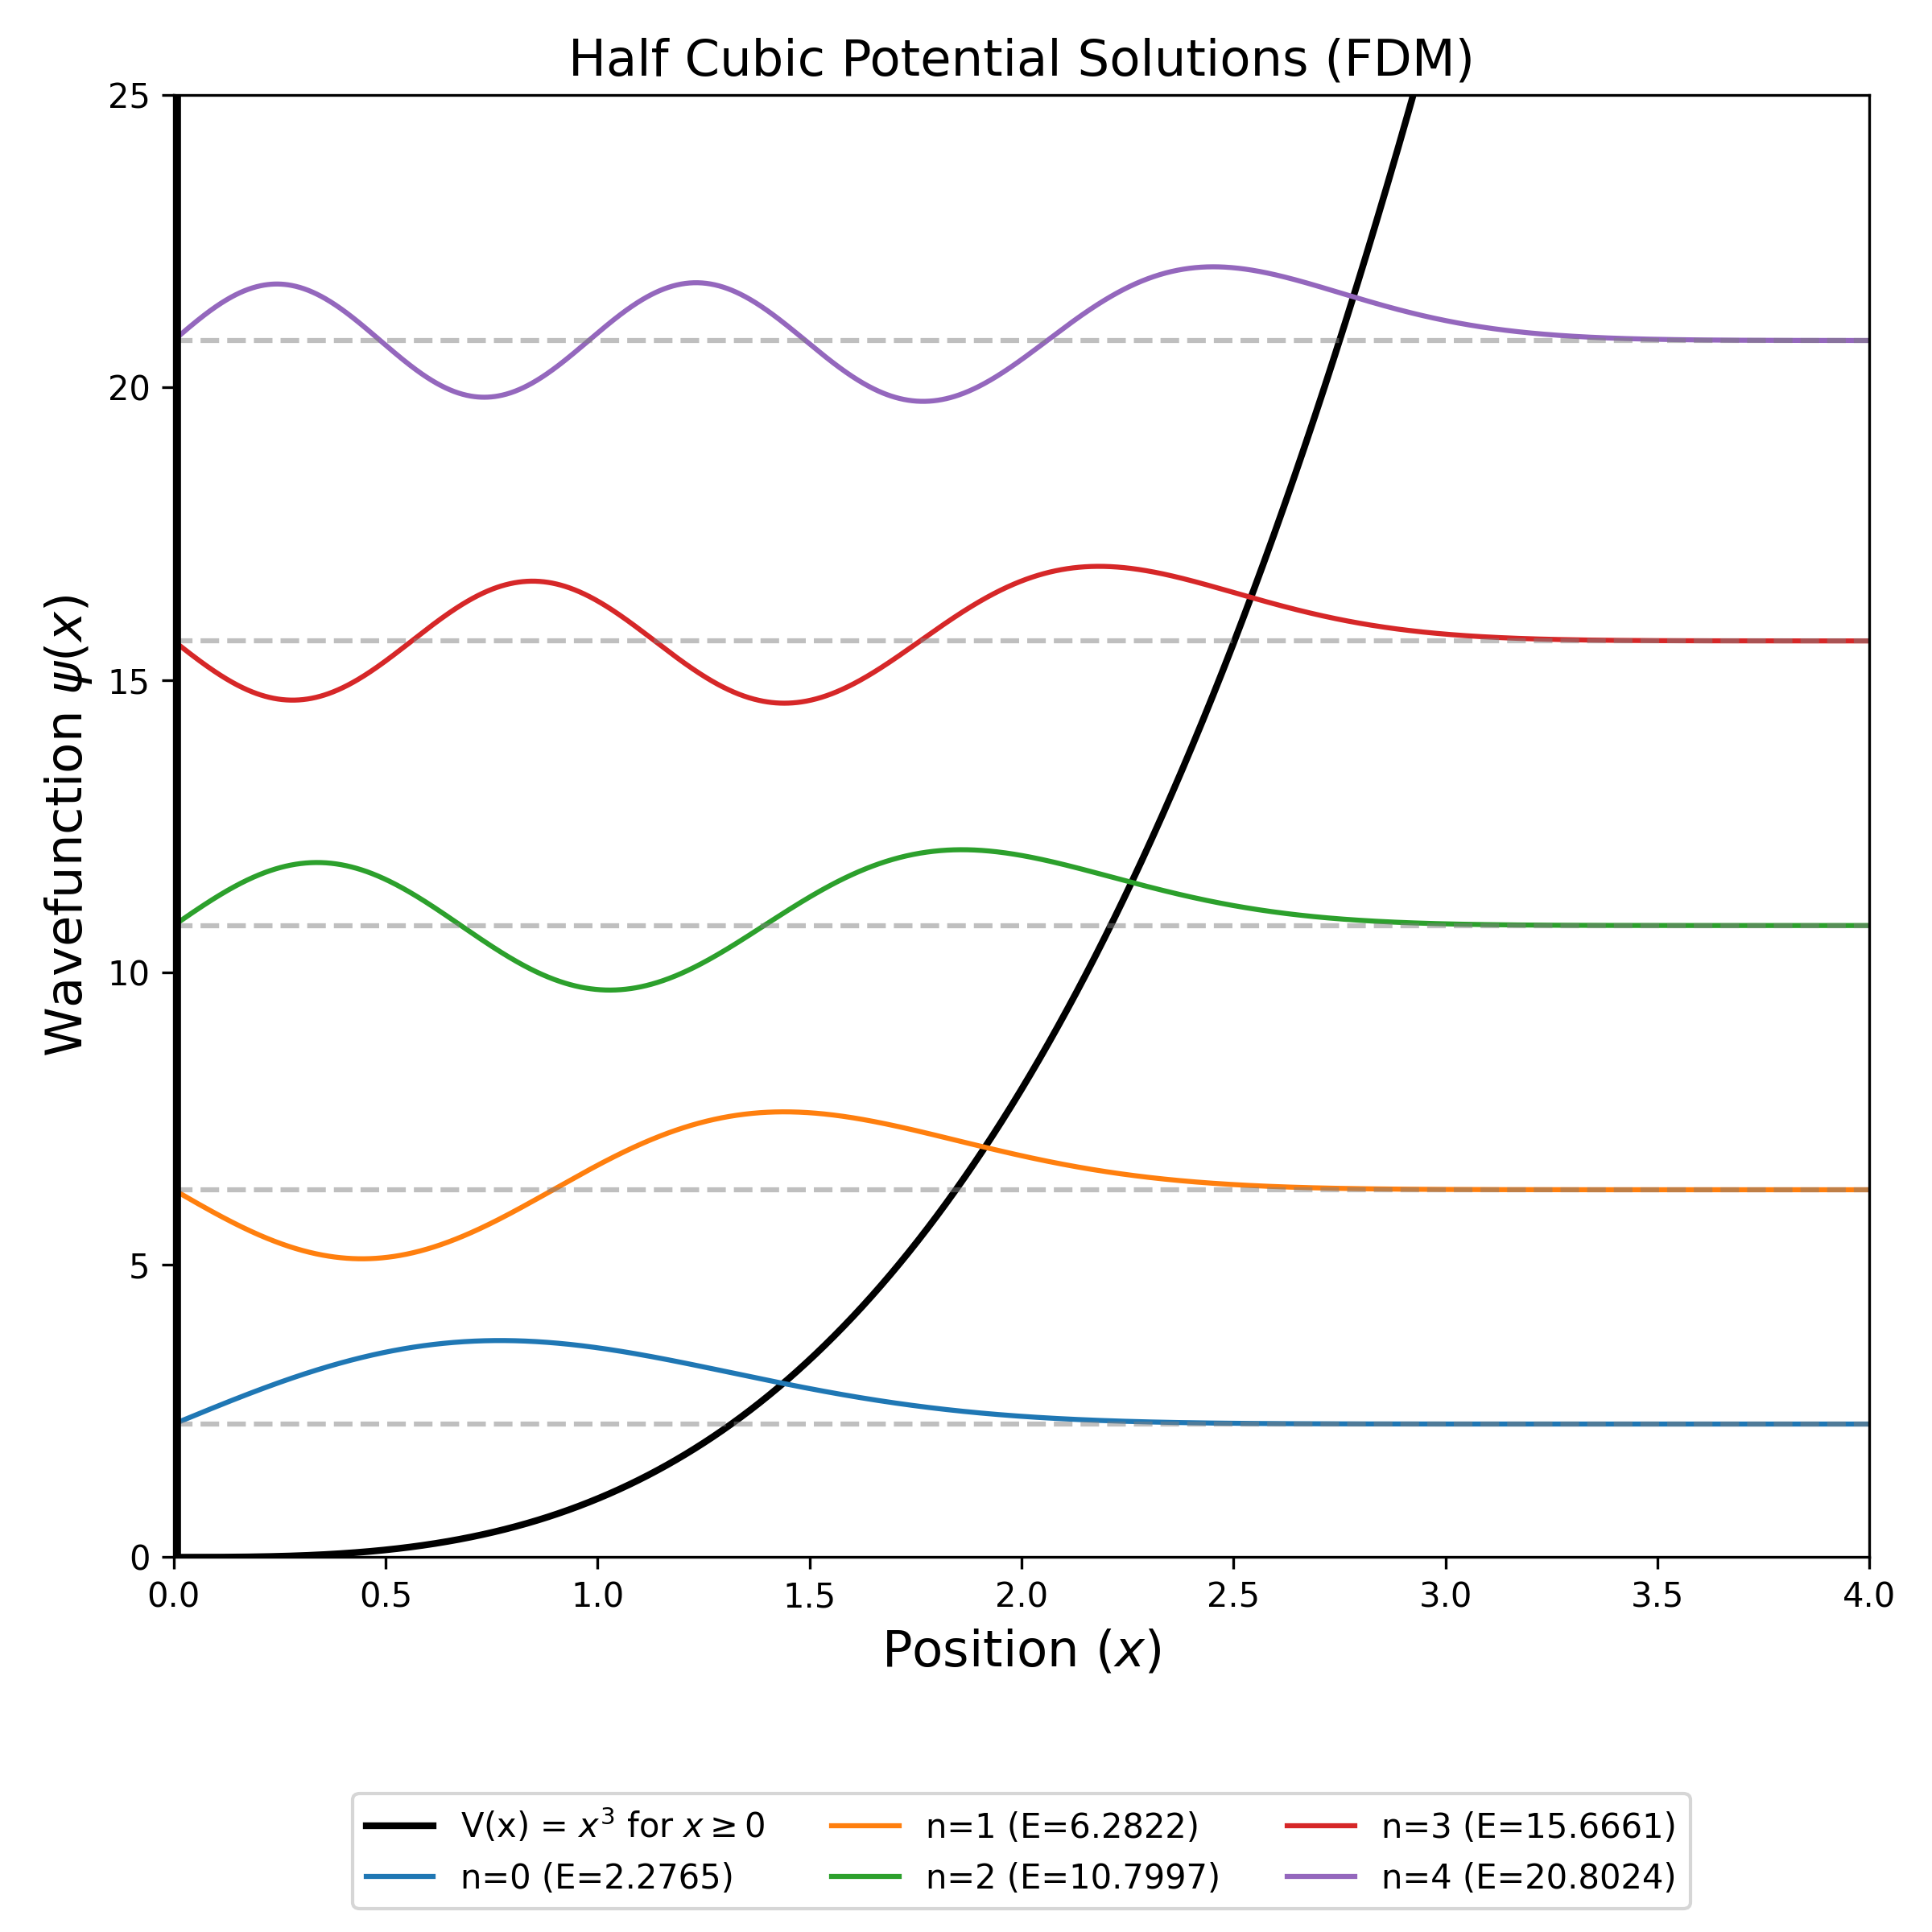
\includegraphics[width=0.8\textwidth]{plots/prob10_half_cubic.png}
            \label{fig:prob10_wavefunction}
            \end{figure}
            \item {\bf Plot Analysis: } Similar to the half-harmonic case, the wavefunctions are strictly zero at $x=0$. The asymmetry of the $x^3$ growth pushes the peaks of the higher excited states further to the right compared to a quadratic well.
        \end{itemize}

        \subsection{Problem 11: Half-Quartic Potential} 
        \begin{itemize}
            \item {\bf Description: } A quartic well bounded by an infinite wall at the origin.
            \item {\bf Potential: } $V(x) = x^4$ when $x \ge 0$, and $\infty$ otherwise.
            \item {\bf Code: } \lstinputlisting[style= codestyle]{src/problems/prob11_half_quartic.f90}
            \item {\bf Output: } \lstinputlisting[style= outputstyle]{output/prob11.txt}
            \item {\bf Plot: }The wavefunctions were visualized using the standard scaling script (defined in Section 2.3) with a visual \texttt{scale\_factor} of 30.0 to prevent overlap between the energy levels.\begin{figure}[H]
            \centering
            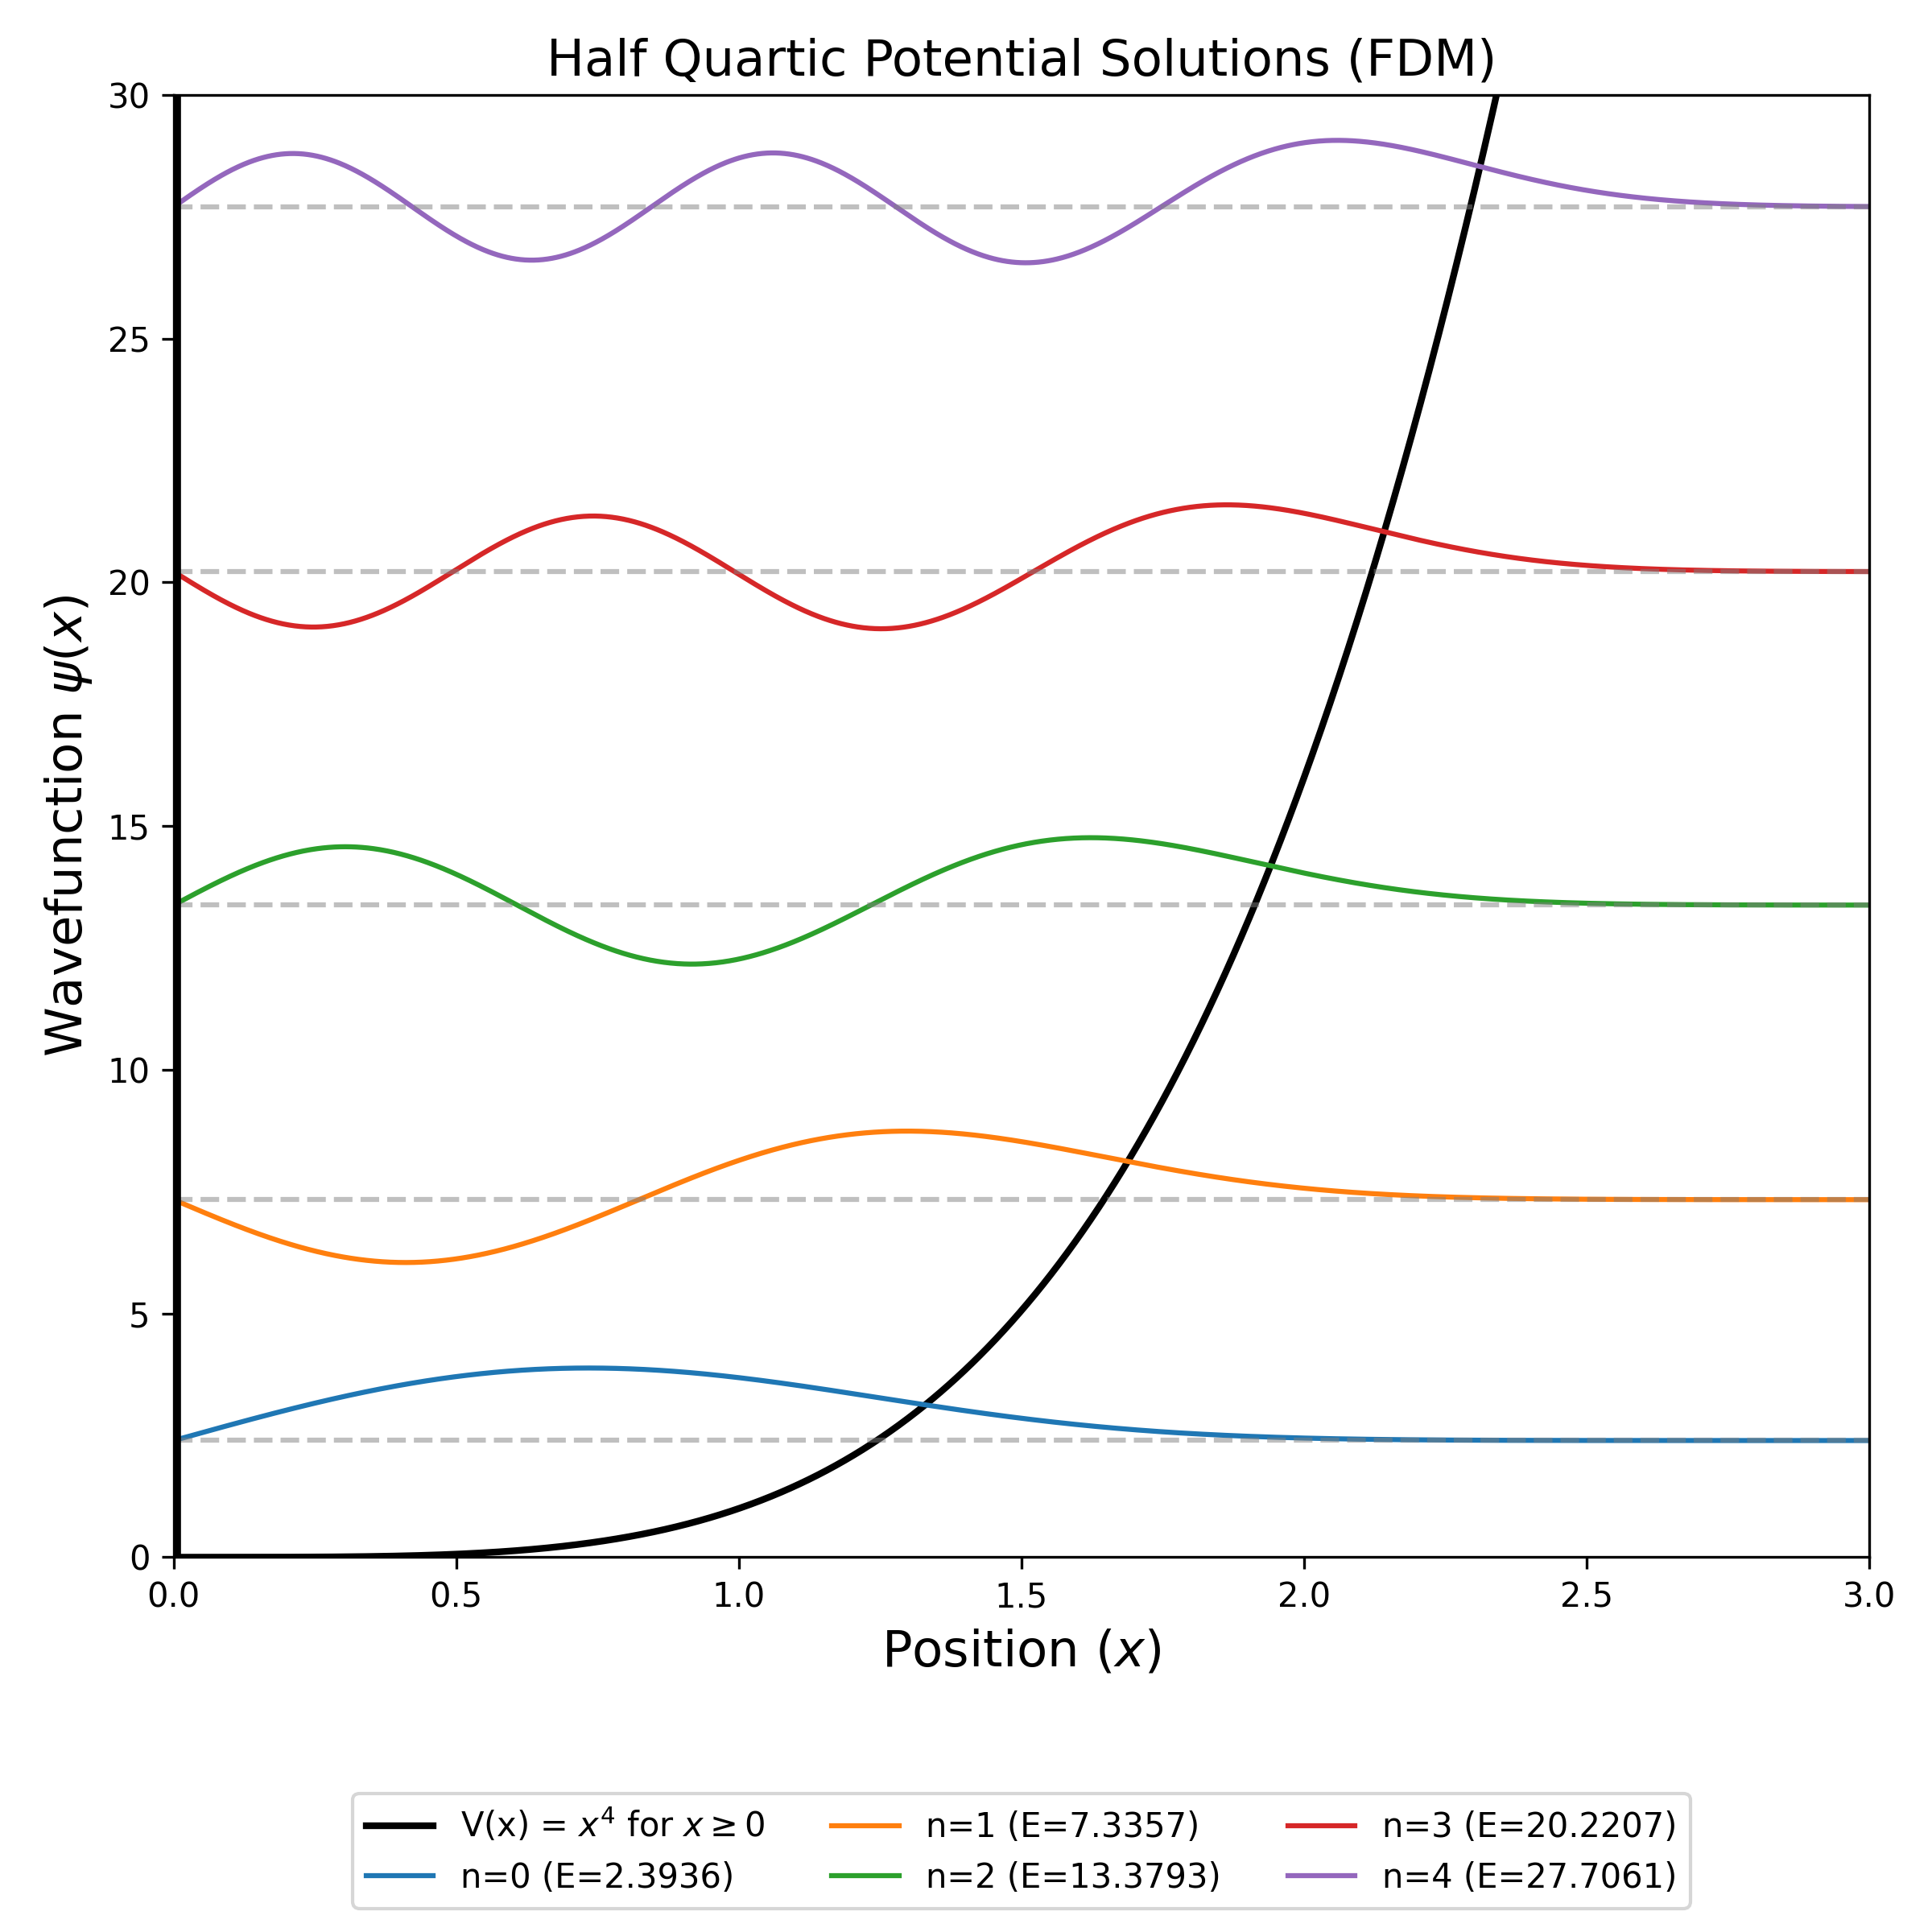
\includegraphics[width=0.8\textwidth]{plots/prob11_half_quartic.png}
            \label{fig:prob11_wavefunction}
            \end{figure}
            \item {\bf Plot Analysis: } Features a highly compressed spatial domain due to the steep $x^4$ rise combined with the hard wall. This leads to highly localized probability densities and widely separated energy eigenvalues.
        \end{itemize}

    \section{Additional Exercises}
        \subsection{Problem 12: Double Well Potential} 
        \begin{itemize}
            \item {\bf Description: } Two deep minima separated by a central potential barrier.
            \item {\bf Potential: } $V(x) = \lambda(x^2 - a^2)^2$ (Used: $V(x) = 0.5(x^2 - 9)^2$).
            \item {\bf Code: } \lstinputlisting[style= codestyle]{src/problems/prob12_double_well.f90}
            \item {\bf Output: } \lstinputlisting[style= outputstyle]{output/prob12.txt}
            \item {\bf Plot: }The wavefunctions were visualized using the standard scaling script (defined in Section 2.3) with a visual \texttt{scale\_factor} of 30.0 to prevent overlap between the energy levels.\begin{figure}[H]
            \centering
            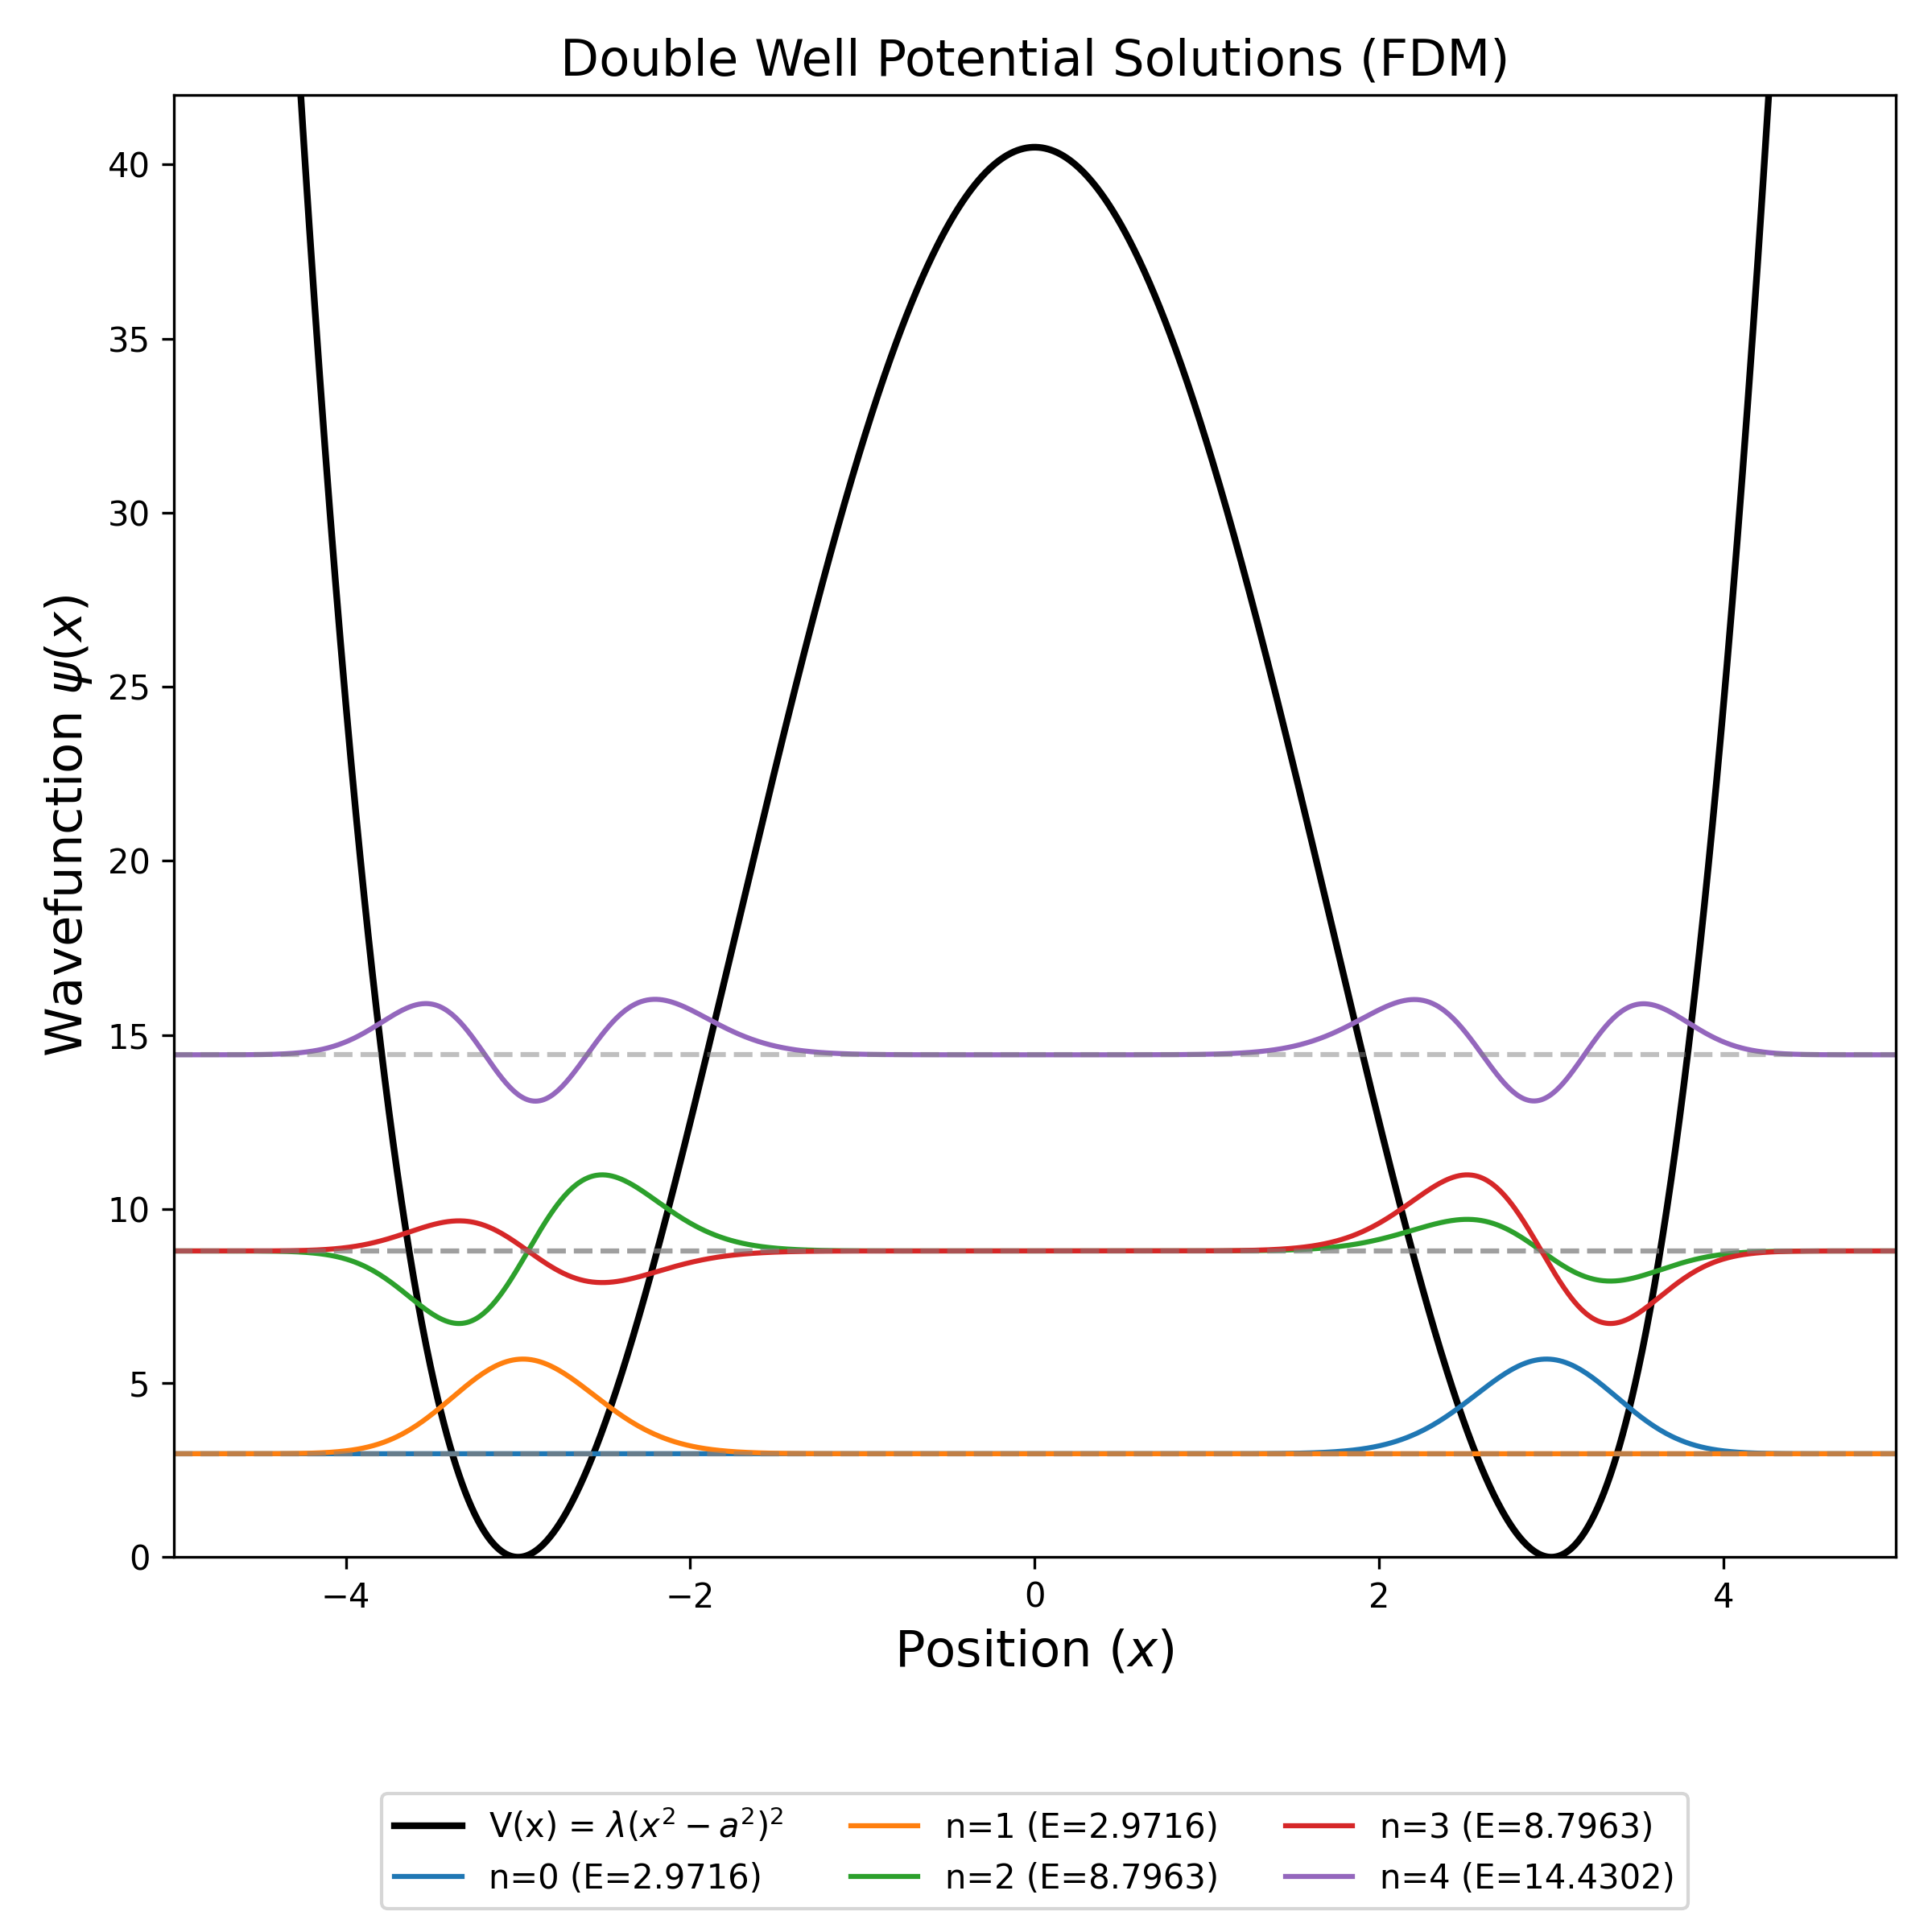
\includegraphics[width=0.8\textwidth]{plots/prob12_double_well_potential.png}
            \label{fig:prob12_wavefunction}
            \end{figure}
            \item {\bf Plot Analysis: } Reveals quantum tunneling. The lowest energy states form almost-degenerate pairs ($E_0 \approx E_1$). The splitting $\Delta E$ is infinitesimally small. Due to the limits of double-precision floating-point arithmetic, the solver exhibits spontaneous symmetry breaking, resolving the states into localized wavefunctions in either the left or right well rather than perfect symmetric/antisymmetric superpositions.
        \end{itemize}

        \subsection{Problem 13: The Morse Potential} 
        \begin{itemize}
            \item {\bf Description: } The Morse potential is a realistic model for the vibrational structure of a diatomic molecule. Unlike the simple harmonic oscillator, which assumes bonds can stretch infinitely without breaking, the Morse potential accurately models molecular dissociation. It features a steep repulsive wall at short distances and flattens out to a finite dissociation energy at large distances.
            \item {\bf Potential: } $V(x) = D_e \left( 1 - e^{-ax} \right)^2$ (Used: $V(x) = 2 \left( 1 - e^{-0.18x} \right)^2$).
            \item {\bf Code: } \lstinputlisting[style= codestyle]{src/problems/prob13_morse_potential.f90}
            \item {\bf Output: } \lstinputlisting[style= outputstyle]{output/prob13.txt}
            \item {\bf Plot: }The wavefunctions were visualized using the standard scaling script (defined in Section 2.3) with a visual \texttt{scale\_factor} of 1.0 to prevent overlap between the energy levels.\begin{figure}[H]
            \centering
            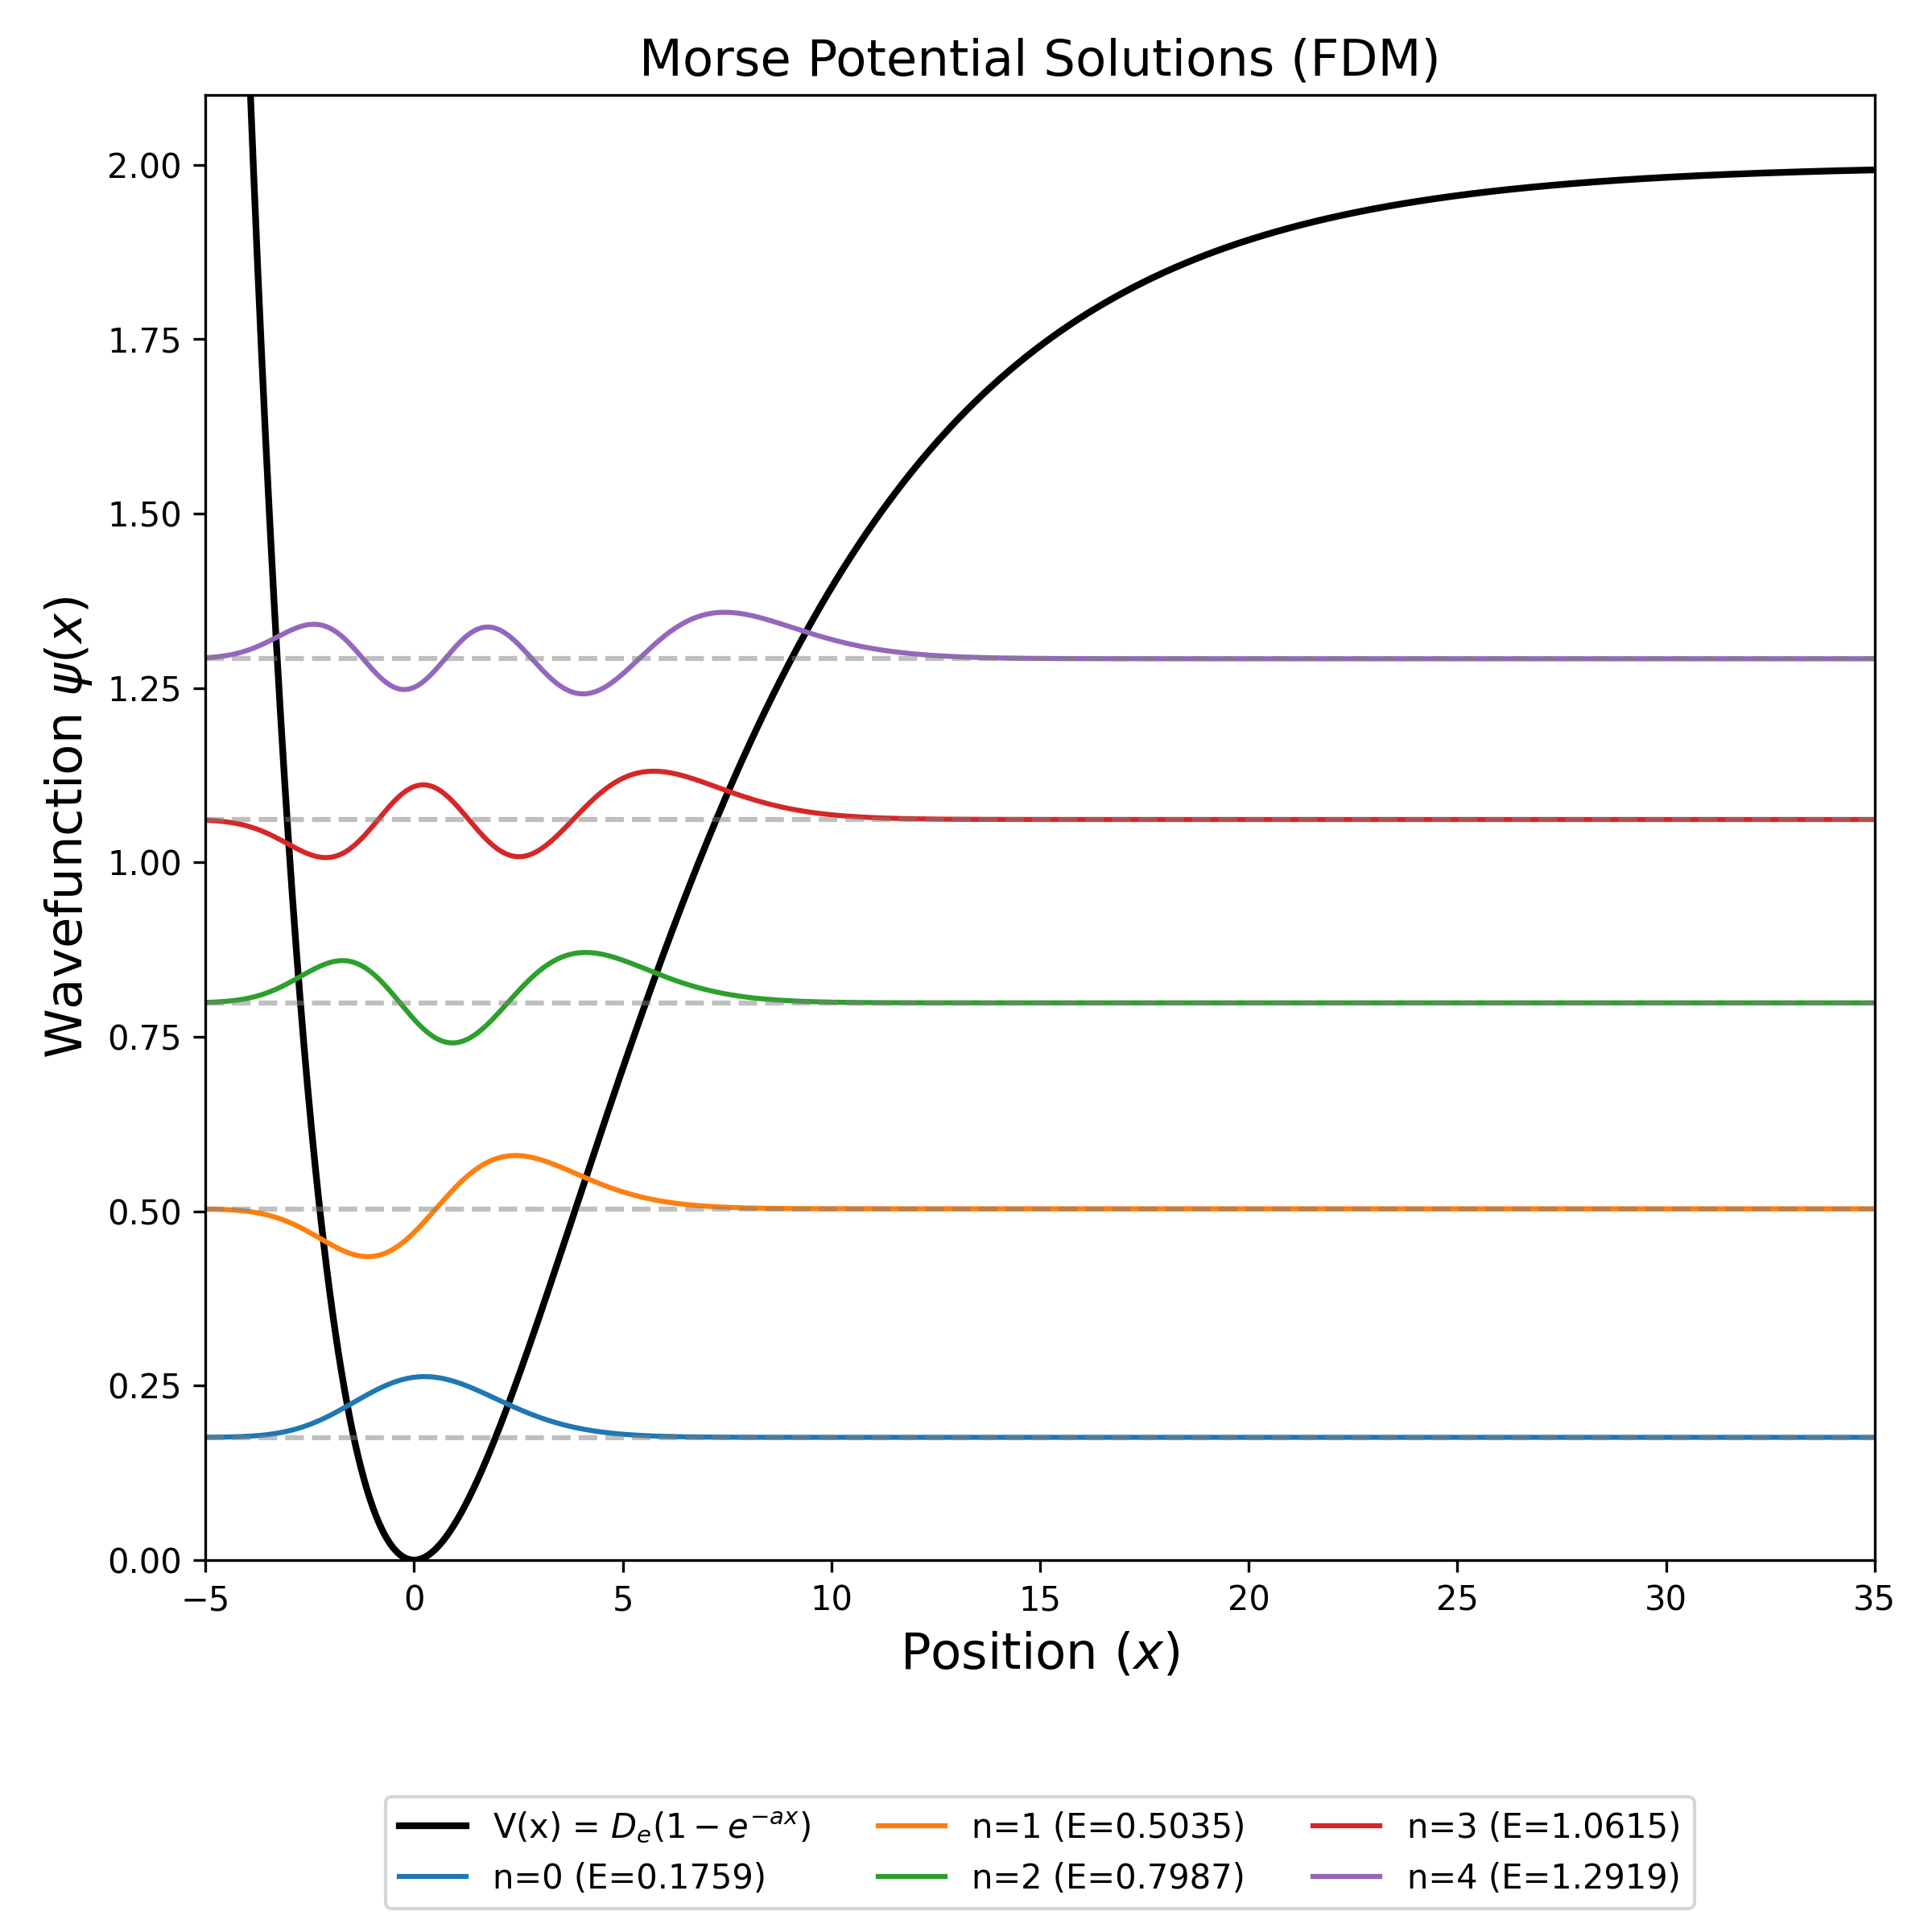
\includegraphics[width=0.8\textwidth]{plots/prob13_morse_potential.png}
            \label{fig:prob13_wavefunction}
            \end{figure}
            \item {\bf Plot Analysis: } The numerical results highlight the anharmonicity of the Morse potential. Unlike the equidistant energy levels of the harmonic oscillator, the calculated energy gaps ($E_{n+1} - E_n$) systematically decrease as the quantum number $n$ increases, representing the weakening of the molecular bond at higher vibrational states.Visually, the wavefunctions exhibit broken symmetry. The left side of the probability distribution is sharply truncated by the steep repulsive wall, while the right side decays slowly, bulging outward into the wide dissociation region.
        \end{itemize}

        \subsection{Problem 14: The Dirac Delta Potential} 
        \begin{itemize}
            \item {\bf Description: } The attractive Dirac delta potential represents an idealized, infinitely deep, and infinitely narrow potential well. It is a critical theoretical test case because it analytically possesses exactly one bound state.
            \item {\bf Potential: } $V(x) = -\alpha \delta(x)$. Because a computer grid cannot evaluate absolute infinity, the delta function is defined via the discrete grid spacing $\Delta x$. The potential is explicitly zero everywhere except at the exact coordinate origin ($x=0$), where it is approximated as: $V(0) = -\frac{\alpha}{\Delta x}$.
            \item {\bf Code: } \lstinputlisting[style= codestyle]{src/problems/prob14_dirac_delta_potential.f90}
            \item {\bf Output: } \lstinputlisting[style= outputstyle]{output/prob14.txt}
            \item {\bf Plot: }The wavefunctions were visualized using the standard scaling script (defined in Section 2.3) with a visual \texttt{scale\_factor} of 20.0 to prevent overlap between the energy levels.\begin{figure}[H]
            \centering
            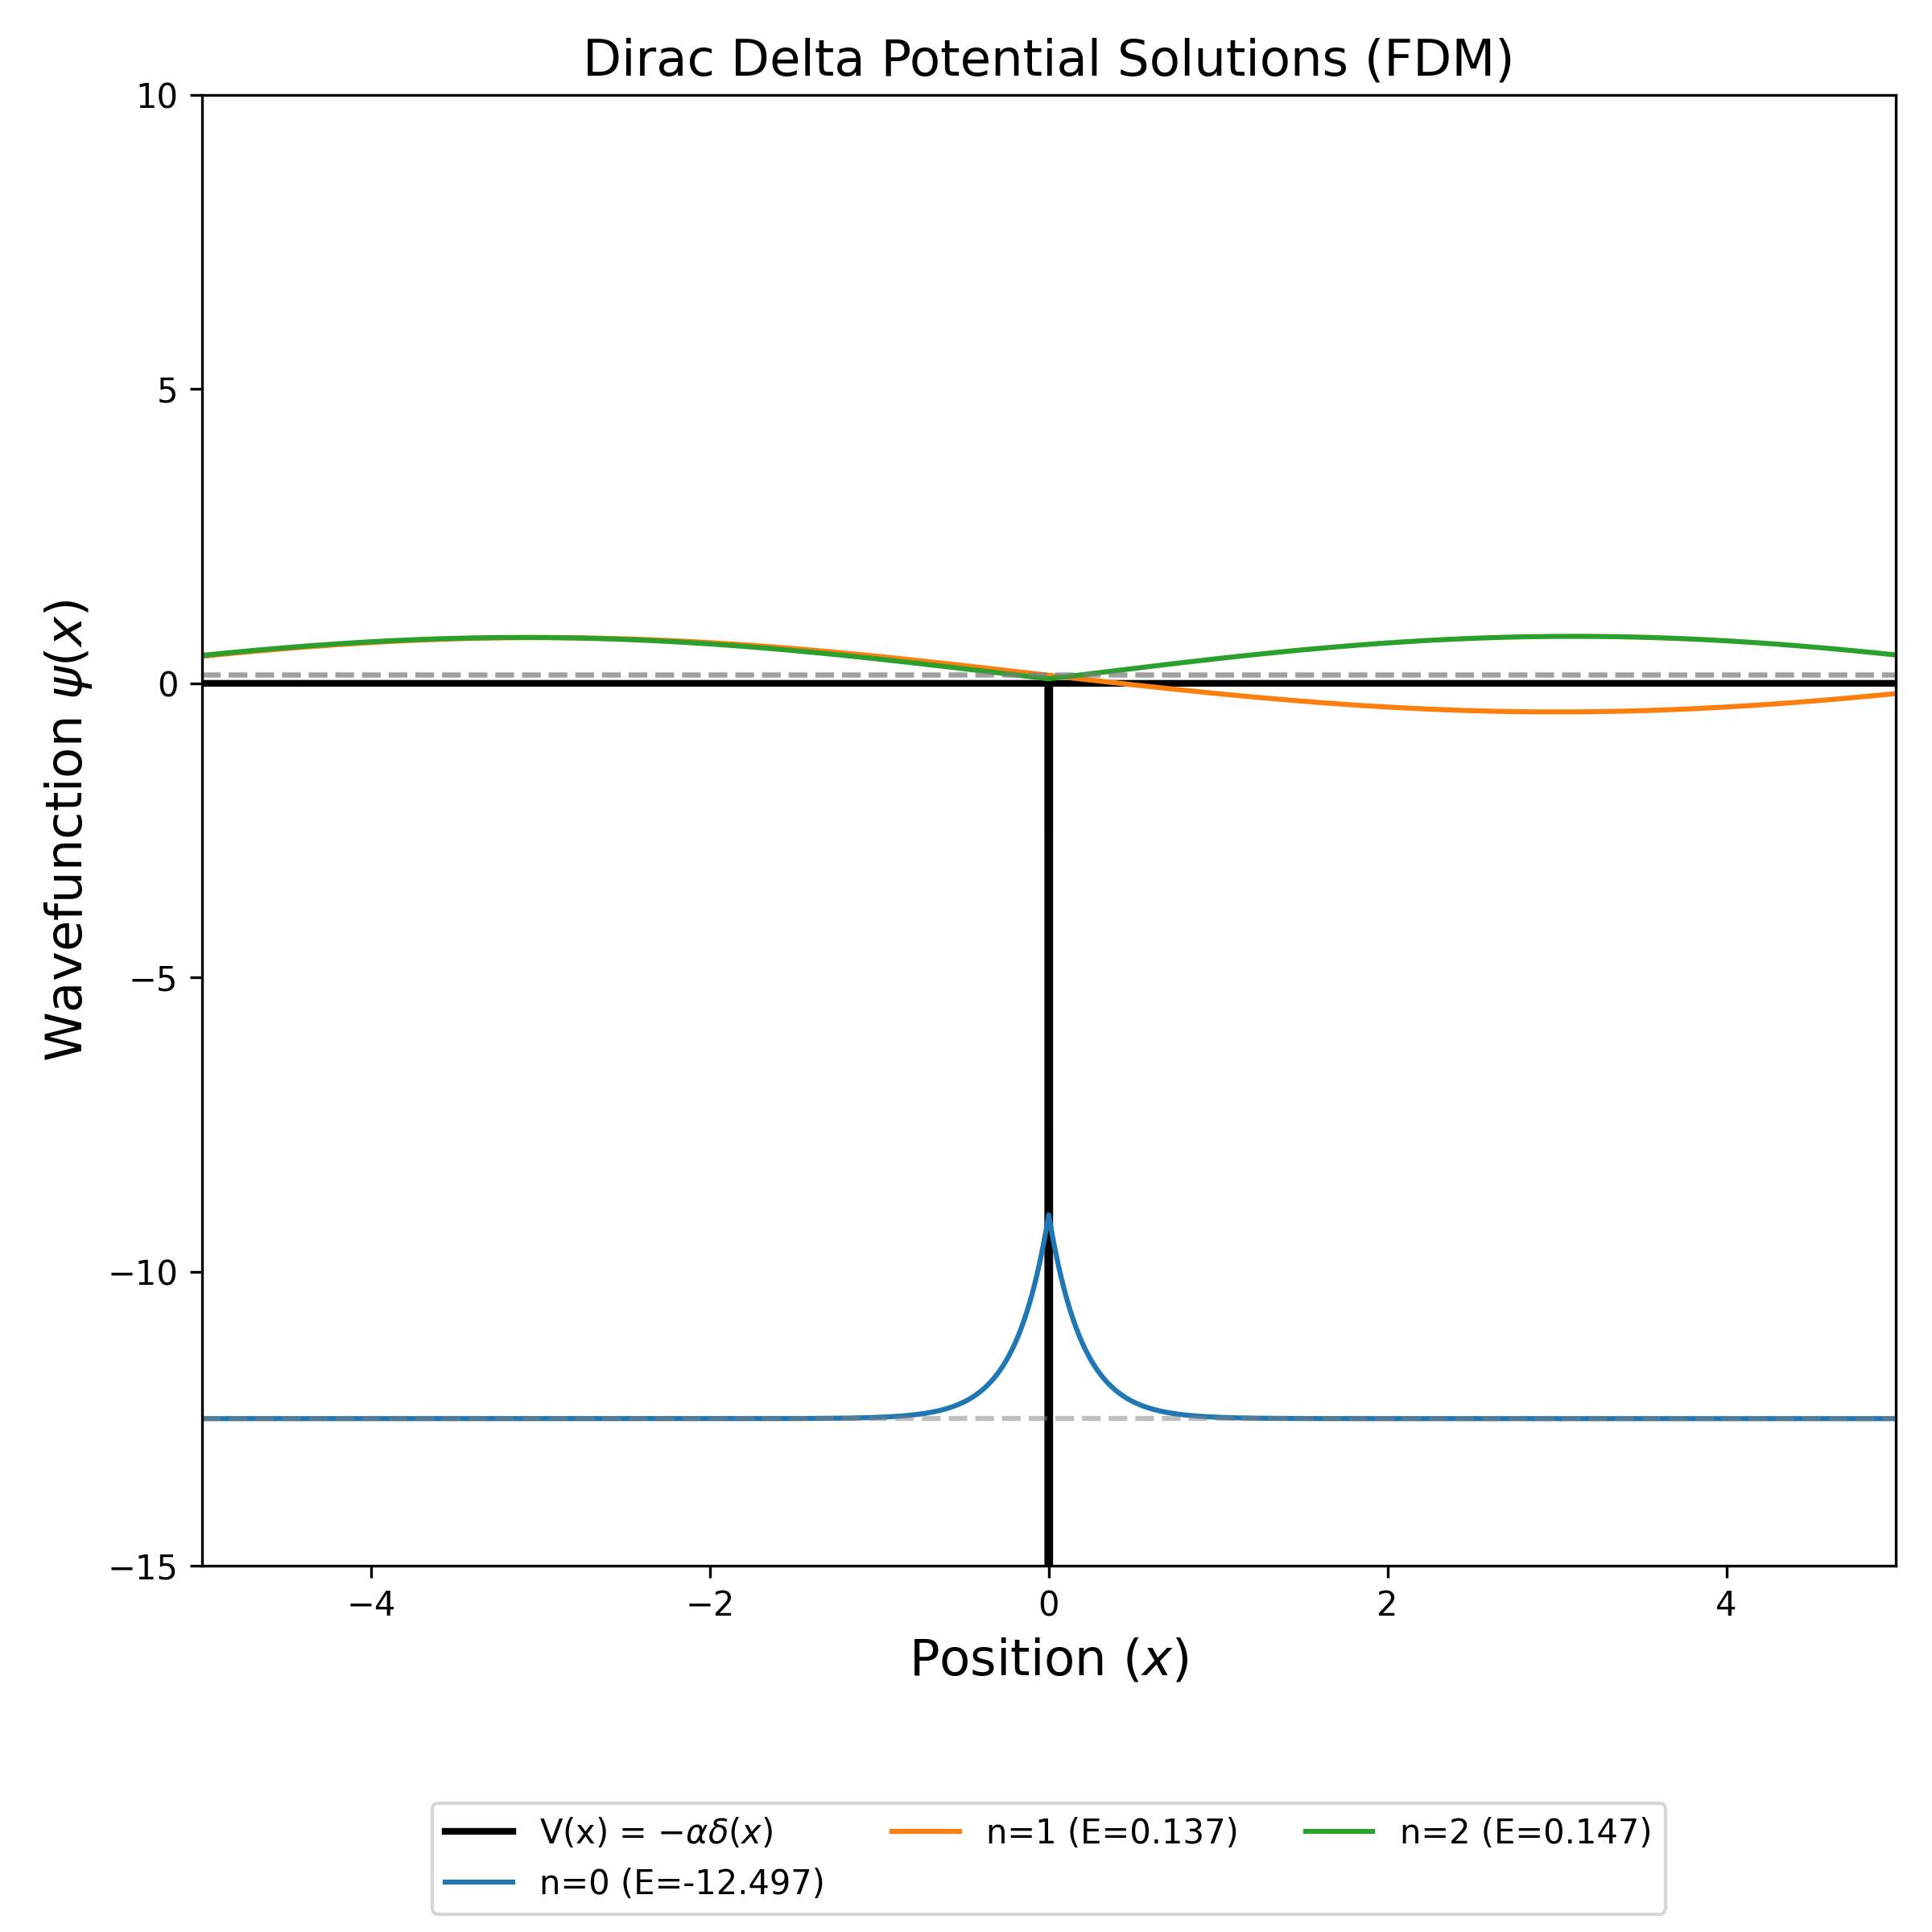
\includegraphics[width=0.8\textwidth]{plots/prob14_dirac_delta_potential.png}
            \label{fig:prob14_wavefunction}
            \end{figure}
            \item {\bf Plot Analysis: } The FDM solver successfully identified the single theoretical bound state ($n=0$, $E_0 < 0$). The ground state wavefunction displays the characteristic sharp, discontinuous cusp at $x=0$ and decays exponentially outward.
            Fascinating numerical artifacts emerge for the excited states ($n > 0$). Because these states possess positive energy ($E > 0$), they are unbound scattering states. In the simulation, they are artificially trapped by the infinite walls of the computational domain $L_{\text{box}}$.
            Notably, the first excited state ($n=1$) possesses odd parity, enforcing a node at the origin ($\psi(0) = 0$). Because the particle's probability density is strictly zero exactly where the delta potential exists, the particle completely ignores the well, resulting in a wavefunction identical to that of a free particle in an infinite square well.
        \end{itemize}
        
        
    \section{Remarks}
    \begin{enumerate}
        \item {\bf Truncation Error: } The central difference approximation for the second derivative introduces an inherent $O(\Delta x^2)$ truncation error. While increasing $N$ reduces this error, it heavily impacts computational time.
        \item {\bf Artificial Boundary Conditions: } For extended potentials (like the finite well or double well), the computational domain $L_{\text{box}}$ must be artificially truncated. If $L_{\text{box}}$ is not sufficiently large, the enforcement of $\psi = 0$ at the grid boundaries acts as an unintended infinite wall, artificially squeezing the wavefunction and raising the calculated energy eigenvalues.
        \item {\bf Numerical Precision Limits: } As observed in the double well potential, standard 64-bit floating-point precision ($\sim 15$ decimal places) can be insufficient to resolve near-degenerate states. When the tunneling splitting drops below numerical noise, algebraic solvers fail to preserve the physical symmetry of the eigenvectors.
    \end{enumerate}
\end{document}